\documentclass[12pt,twoside]{report}
% Pengaturan ukuran halaman dan margin
\usepackage[a4paper,top=30mm,left=30mm,right=20mm,bottom=25mm]{geometry}

% Pengaturan ukuran spasi
\usepackage[singlespacing]{setspace}

% Pengaturan jenis karakter
\usepackage[utf8]{inputenc}

% Pengaturan pewarnaan
\usepackage[table,xcdraw]{xcolor}

% Pengaturan kutipan artikel
\usepackage[style=apa, backend=biber]{biblatex}

% Package lainnya
\usepackage{graphicx,tabularx,multirow}
\usepackage[bahasa]{babel}
\usepackage{changepage}
\usepackage{enumitem}
\usepackage{eso-pic}
\usepackage{txfonts} % Font times
\usepackage{etoolbox}
\usepackage{graphicx}
\usepackage{lipsum}
\usepackage{longtable}
\usepackage{tabularx}
\usepackage{wrapfig}
\usepackage{float}
\usepackage{gensymb}
\usepackage[colorlinks=true, linkcolor=black, citecolor=black, urlcolor=blue]{hyperref}

% Pengaturan jenis karakter
\usepackage[utf8]{inputenc}

% Pengaturan format daftar isi, daftar gambar, dan daftar tabel
\usepackage[titles]{tocloft}
\setlength{\cftsecindent}{2em}
\setlength{\cftsubsecindent}{2em}
\setlength{\cftbeforechapskip}{1.5ex}
\setlength{\cftbeforesecskip}{1.5ex}
\setlength{\cftbeforetoctitleskip}{0cm}
\setlength{\cftbeforeloftitleskip}{0cm}
\setlength{\cftbeforelottitleskip}{0cm}
\renewcommand{\cfttoctitlefont}{\hfill\Large\bfseries} % command untuk membuat heading bold dan besar
\renewcommand{\cftaftertoctitle}{\hfill}
\renewcommand{\cftloftitlefont}{\hfill\Large\bfseries}
\renewcommand{\cftafterloftitle}{\hfill}
\renewcommand{\cftlottitlefont}{\hfill\Large\bfseries}
\renewcommand{\cftafterlottitle}{\hfill}

% Pengaturan format judul bab
\usepackage{titlesec}
\renewcommand{\thesection}{\thechapter.\arabic{section}}
\titleformat{\chapter}[display]{\centering\bfseries\large}{Modul\ \arabic{chapter}\ }{0ex}{\vspace{0ex}\centering}
\titleformat*{\section}{\large\bfseries}
\titleformat*{\subsection}{\normalsize\bfseries}
\titlespacing{\chapter}{0ex}{0ex}{4ex}
\titlespacing{\section}{0ex}{1ex}{0ex}
\titlespacing{\subsection}{0ex}{0.5ex}{0ex}
\titlespacing{\subsubsection}{0ex}{0.5ex}{0ex}
\setcounter{secnumdepth}{3} % Untuk memberi penomoran pada \subsubsection

\patchcmd{\cleardoublepage}{\hbox{}}{
  \thispagestyle{empty}
  \vspace*{\fill}
  \begin{center}\textit{[Halaman ini sengaja dikosongkan]}\end{center}
  \vfill}{}{}

\counterwithin{figure}{chapter}
\counterwithin{table}{chapter}

\definecolor{visigrey}{rgb}{.1,.15,.15}
\geometry{top=1cm,bottom=.5cm}
\savegeometry{titlepage}
\geometry{top=2cm,bottom=2cm}
\savegeometry{main}

\def\bspace{\(\qquad\qquad\qquad\)}
\usepackage[T1]{fontenc}
\usepackage{tgheros}
\renewcommand*\familydefault{\sfdefault}

\setcounter{tocdepth}{6}

\def\autor{Laboratorium }
\def\lab{Robotika dan Sistem Cerdas}
\def\departemen{Departemen Teknik Komputer}
\def\institut{Institut Teknologi Sepuluh Nopember}
\def\praktikum{Praktikum \\ Workshop Telematika}
\def\judul{Modul}
\def\tahun{2023}



\begin{document}
	  % Ubah Bahasa sesuai dengan keinginan
    \selectlanguage{bahasa}
    
    % Nomor halaman pembuka dimulai dari sini
    \pagenumbering{roman}

    % Atur ulang penomoran halaman
    \setcounter{page}{1}

    \def\headingtype{\bf \small}
\loadgeometry{titlepage}
\begin{titlepage}
	\centering
	\begin{tabularx}{\textwidth}{Xr}
		\multirow[c]{6}{*}{
\includegraphics[width=3cm]{Cover/img/logodepart.png}}	 & {\emph{\headingtype \autor}} \\ [-2pt]
		&	{\headingtype \lab} \\[-2pt]
		&	{\headingtype \departemen} \\[-2pt]
		&	{\headingtype \emph{\institut}} \\[-2pt]	
		\vspace{1.6cm}
	\end{tabularx}\par
	\vspace{5.0cm}
	{\Huge \bf  \praktikum \par}
	\vspace{2.0cm}
	{\LARGE \bf \judul \par}
	\vspace{2.0cm}
	{\Large \tahun \par}
	\vfill
	{\centering
		
\includegraphics[width=\textwidth]{Cover/img/footer.png}
	}
\end{titlepage}
\loadgeometry{main}
    \cleardoublepage
    
    \setlist[itemize]{itemsep=0pt, parsep=0pt} % Untuk itemize
    \setlist[enumerate]{itemsep=0pt, parsep=0pt} % Untuk enumerate

    \begin{spacing}{1.5}
        % Daftar isi
        \renewcommand*\contentsname{DAFTAR ISI}
        \addcontentsline{toc}{chapter}{\contentsname}
        \tableofcontents
        \cleardoublepage
    
        % Daftar gambar
        \renewcommand*\listfigurename{DAFTAR GAMBAR}
        \addcontentsline{toc}{chapter}{\listfigurename}
        \listoffigures
        \cleardoublepage
    
        % Daftar tabel
        \renewcommand*\listtablename{DAFTAR TABEL}
        \addcontentsline{toc}{chapter}{\listtablename}
        \listoftables
        \cleardoublepage
    \end{spacing}
    % Nomor halaman isi dimulai dari sini
    \pagenumbering{arabic}
    \setcounter{page}{1}
  \linespread{1.25}
	\chapter{Dasar Telematika}

\section{Tujuan}
\begin{enumerate}
    \item Belajar menyusun dan menganalisa rangkaian
    \item Mengetahui fungsi setiap komponen dan cara implementasinya
    \item Untuk memperkenalkan beberapa konsep dasar dan teknik laboratorium dalam bekerja menggunakan peralatan elektronika dan soldering
\end{enumerate}

\section{Dasar Teori}
Seven Segment Display memiliki 7 Segmen dimana setiap segmen dikendalikan secara ON dan OFF untuk menampilkan angka yang diinginkan. 
Angka-angka dari 0 (nol) sampai 9 (Sembilan) dapat ditampilkan dengan menggunakan beberapa kombinasi Segmen. Selain 0 – 9, Seven Segment 
Display juga dapat menampilkan Huruf Hexadecimal dari A sampai F. Segmen atau elemen-elemen pada Seven Segment Display diatur menjadi 
bentuk angka “8” yang agak miring ke kanan dengan tujuan untuk mempermudah pembacaannya. Pada beberapa jenis Seven Segment Display, 
terdapat juga penambahan “titik” yang menunjukan angka koma decimal.  Terdapat beberapa jenis Seven Segment Display, diantaranya adalah 
Incandescent bulbs, fluorescent lamps (FL), Liquid Crystal Display (LCD) dan Light Emitting Diode (LED).

Salah satu jenis Seven Segment Display yang sering digunakan adalah 7 Segmen yang menggunakan LED (Light Emitting Diode) sebagai penerangnya.  
LED 7 Segmen ini umumnya memiliki 7 Segmen atau elemen garis dan 1 segmen titik yang menandakan “koma” Desimal. Jadi Jumlah keseluruhan segmen 
atau elemen LED sebenarnya adalah 8. Cara kerjanya pun boleh dikatakan mudah, ketika segmen atau elemen tertentu diberikan arus listrik, maka 
Display akan menampilkan angka atau digit yang diinginkan sesuai dengan kombinasi yang diberikan.

Logam yang biasa digunakan adalah timah yang memiliki titik leleh antara 90 hingga 450 \degree C. Timah dapat dilelehkan menggunakan solder yang dipanaskan. 
Ketika lelehan timah ini mendingin dan mengeras akan membentuk saluran yang dapat dilalui oleh listrik.  Soldering biasa dilakukan pada PCB (Printed Circuit Board) 
dimana pada PCB terdapat lubang-lubang kecil dimana kaki komponen dapat dimasukan kemudian kaki komponen dapat disolder untung memasang komponen tersebut.

Teknik soldering merupakan proses penggabungan dua komponen logam dengan menggunakan timah solder yang dicairkan untuk membentuk sambungan yang konduktif. 
Proses ini umumnya digunakan dalam industri elektronik untuk menghubungkan komponen pada papan sirkuit. Dalam keadaan di mana sambungan perlu diperbaiki 
atau komponen diganti, teknik desoldering diterapkan. Desoldering adalah proses penghapusan solder dari suatu sambungan untuk melepaskan komponen dari papan sirkuit. 
Kedua teknik ini memerlukan alat khusus, presisi, dan keahlian untuk memastikan sambungan yang efektif dan untuk mencegah kerusakan pada papan atau komponen.


\section{Tugas Pendahuluan}
\begin{enumerate}
    \item Jelaskan bagaimana cara kontrol 7-segment anoda dan katoda?
    \item Buat schematic di Tinkercad untuk menampilkan nomor kelompok menggunakan dua 7-segment!
    \item Install aplikasi Fusion untuk persiapan modul 2!
\end{enumerate}

\section{Alat dan Komponen}
\subsection{Alat}
\begin{enumerate}
    \item Soldering kit
    \item Timah 0.8 mm
    \item Power source
    \item Sikat 
    \item IPA (Isopropyl alcohol)
    \item Flux
    \item Solder Pasta
\end{enumerate}

\subsection{Komponen}
\begin{enumerate}
    \item PCB 4x6 cm                        (1x)
    \item Header Female                     (1x)
    \item Resistor 330-ohm 			        (1x)
    \item White Housing 2 Pin			    (1x)
    \item 7-Segment 0.56-inch Common Katoda	(2x)
    \item Modul LED Chaser kit              (1x)
\end{enumerate}
\section{Eksperimen 1: Teknik Desoldering}
\begin{enumerate}
    \item Dokumentasikan pcb yang akan di desolder.
    \item Siapkan semua peralatan yang disebutkan dan panaskan solder terlebih dahulu
        \begin{figure}[H]
            \centering
            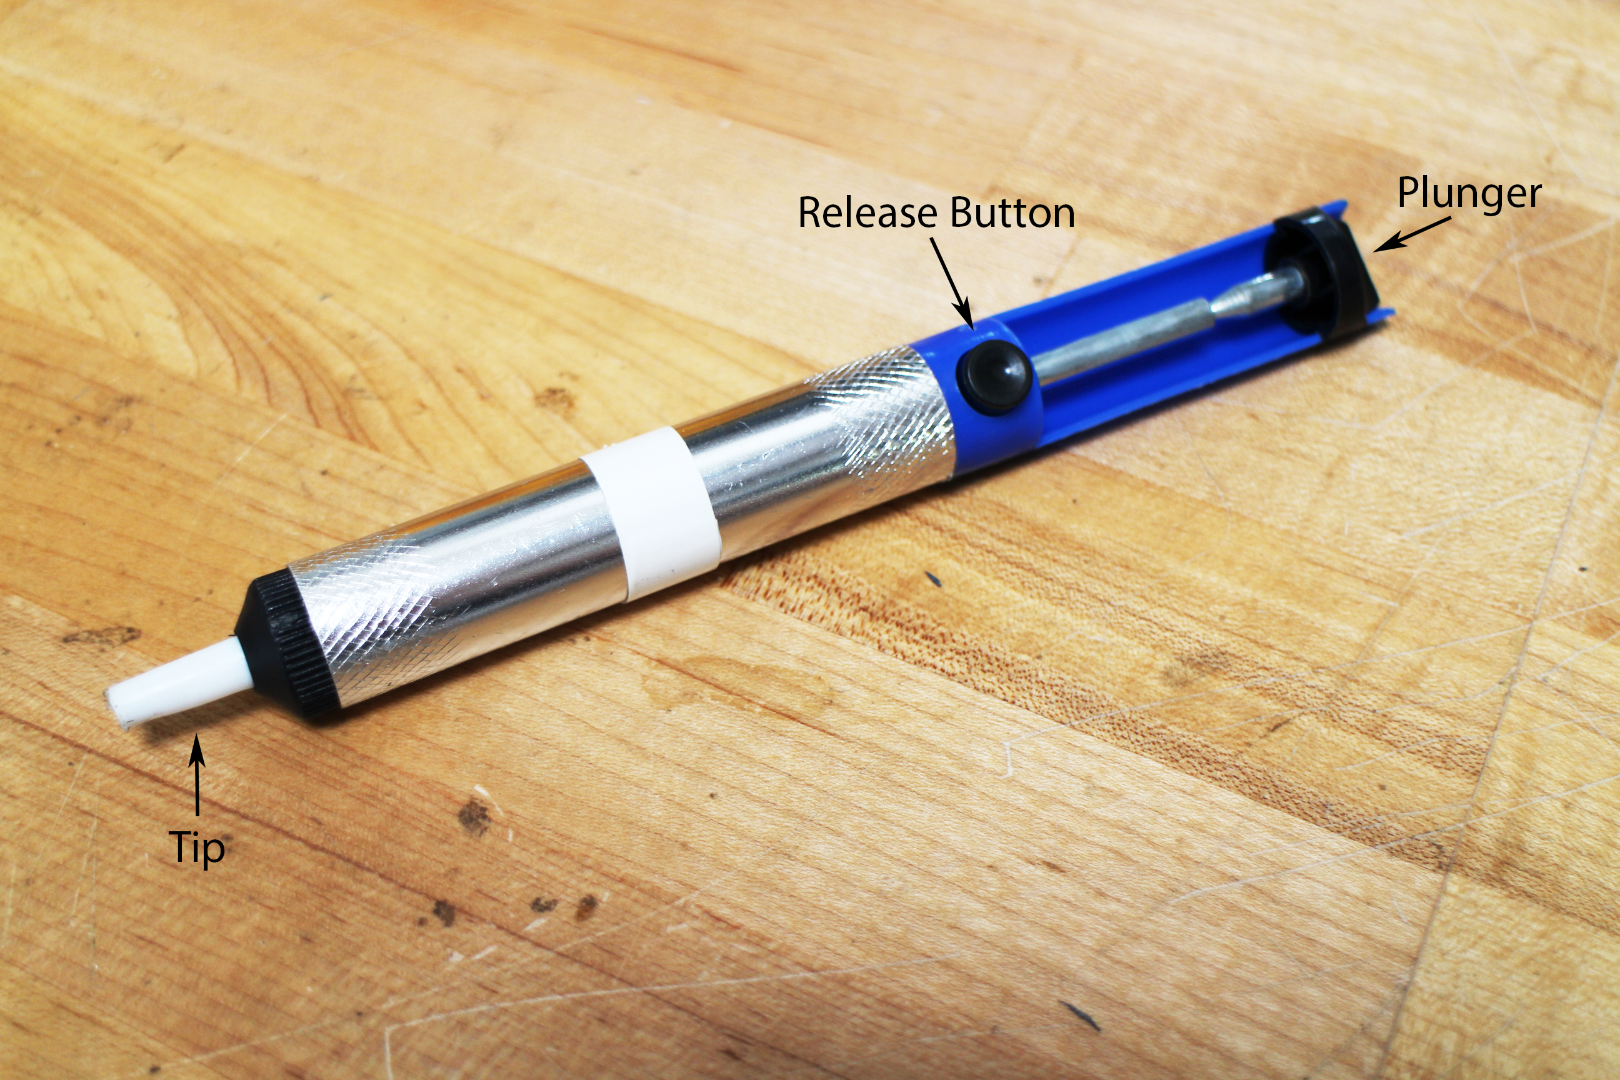
\includegraphics[width=0.6\linewidth]{P1/img/desolder.png}
            \caption{Desolder}
            \label{fig:desolder}
        \end{figure}
    \item Panaskan timah yang ingin  dilepaskan dengan besi solder
    \item Tekan plunger.
    \item Setelah timah menjadi cair, letakkan ujung pompa desolder tepat pada timah yang ingin dilepaskan.
    \item Lepaskan plunger dengan menekan penahan (release button).
    \item Lepaskan komponen yang bebas.
    \item Ulangi langkah 2-6 untuk menghilangkan timah berlebih.
    \item Buang timah di dalam pompa dengan terus menekan dan melepaskan plunger.
    \item Amati output yang dihasilkan, dokumentasikan hasil output dalam bentuk lampiran
\end{enumerate}
\section{Eksperimen 2: Teknik Soldering}
\begin{figure}[H]
    \centering
    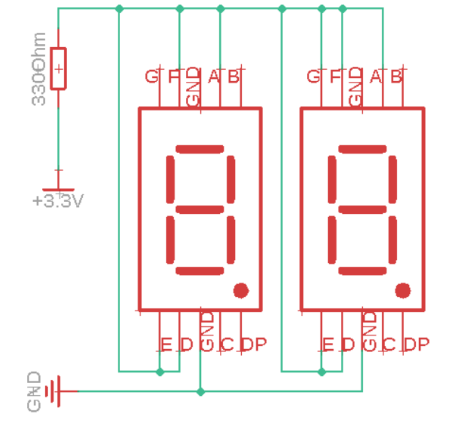
\includegraphics[width=0.4\linewidth]{P1/img/schematics.png}
    \caption{Schematics 7-Segment}
    \label{fig:schematics7Segment}
\end{figure}

\begin{figure}[H]
    \centering
    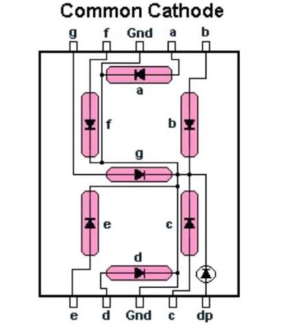
\includegraphics[width=0.4\linewidth]{P1/img/7segment.png}
    \caption{Pin Referensi 7-Segment Katoda}
    \label{fig:Referensi7Segment}
\end{figure}
\begin{enumerate}
    \item Siapkan semua peralatan yang disebutkan dan panaskan solder terlebih dahulu
    \item Pasang header untuk 7-segment pada PCB lalu disolder menggunakan timah. (Pastikan Header terpasang dengan jarak yang sesuai dengan panjang 7-segment).
    \item Kaki-kaki dari komponen  elektronik yang terpasang di pcb dihadapkan ke atas, dan jika kaki-kaki tersebut panjang maka bisa dibengkokkan sehingga saat hendak disolder komponen tersebut tidak rentan bergoyang yang nantinya menyusahkan proses menyolder
    \item Tambahkan pasta fluks pada area copper pad secukupnya, untuk instruksi menyolder bisa diperhatikan di gambar berikut
        \begin{figure}[H]
            \centering
            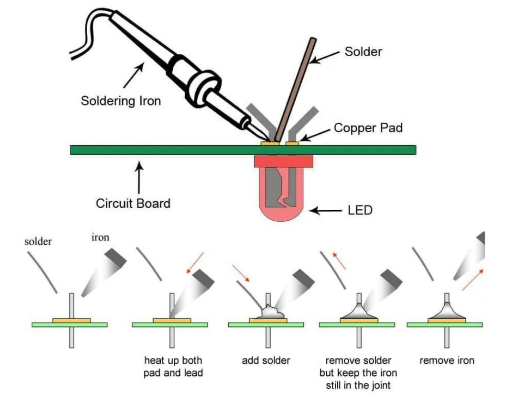
\includegraphics[width=0.6\linewidth]{P1/img/solder1.png}
            \caption{Prosedur Soldering (1)}
            \label{fig:ProsedurSoldering1}
        \end{figure}
        \begin{figure}[H]
            \centering
            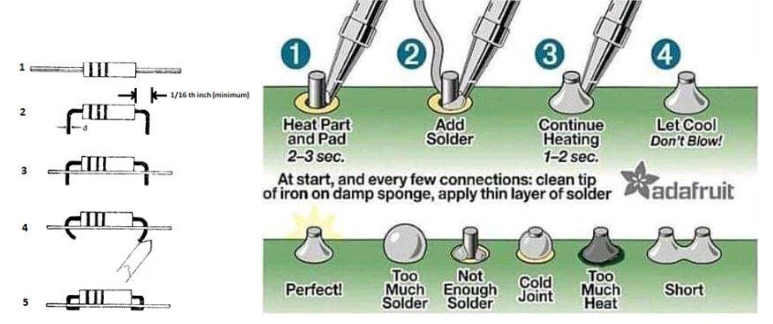
\includegraphics[width=0.8\linewidth]{P1/img/solder2.png}
            \caption{Prosedur Soldering (2)}
            \label{fig:ProsedurSoldering2}
        \end{figure}
    \item Letakkan soldering iron ke permukaan copper pad dan kaki dari komponen yang hendak disolder sehingga panasnya menyebar. Agar panas dari soldering iron lebih cepat menyebar ke copper pad dan kaki komponen, tambahkan sedikit timah ke bagian soldering iron 
    yang nantinya berkontak sehingga luas permukaan penghantar panas bertambah dan proses menyolder menjadi relatif lebih mudah
    \item Setelah copper pad dan kaki komponen dirasa cukup panas, tambahkan timah solder ke arah tersebut hingga timah meleleh dan terbentuk seperti cone kerucut seperti di peraga, lalu angkat timah solder dan soldering iron secara berturut-turut
    \item Gunakan modul 7-segment dan hubungkan rangkaian menggunakan timah yang dipanaskan dengan solder sesuai schematic diatas, lakukanlah proses menyolder ini ke semua komponen elektronik yang diperlukan
    \item Di akhir proses meyolder, seringkali terdapat bekas pasta fluks yang membuat pcb terlihat kurang bersih, untuk membersihkannya gunakan sikat gigi yang dibasahi atau dicelupkan ke IPA dan gosokkan secara searah ke pcb yang dirasa kotor oleh sisa pasta fluks hingga dirasa cukup bersih
    \item Setelah semua komponen terhubung sesuai intruksi, nyalakan power source untuk mencoba rangkaian. Sebelumnya Periksa hasil solder dengan multimeter untuk mengecek konektivitas antar sambungan
    \item Amati output yang dihasilkan, dokumentasikan hasil output dalam bentuk lampiran
        \\ Contoh hasil
        \begin{figure}[H]
            \centering
            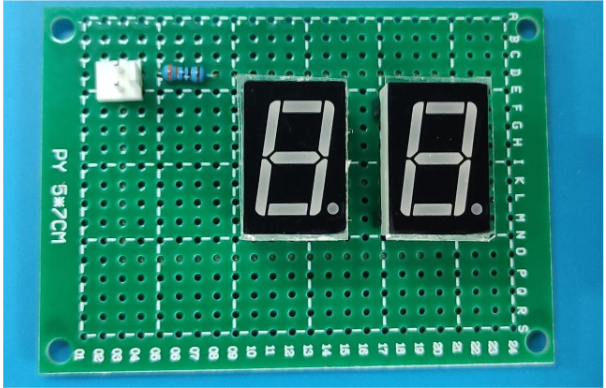
\includegraphics[width=0.8\linewidth]{P1/img/contohhasil1.png}
            \caption{Hasil Soldering Tampak Depan}
            \label{fig:HasilTampakDepan}
        \end{figure}
        \begin{figure}[H]
            \centering
            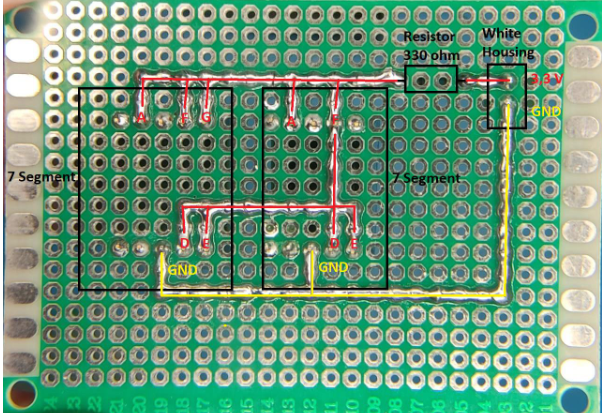
\includegraphics[width=0.8\linewidth]{P1/img/contohhasil2.png}
            \caption{Hasil Soldering Tampak Belakang}
            \label{fig:HasilTampakBelakang}
        \end{figure}
\end{enumerate}

\section{Eksperimen 3: Teknik Soldering Uap}
\subsection{Percobaan 1: Penyolderan SMD}
\begin{enumerate}
    \item Siapkan semua peralatan dan komponen yang dibutuhkan.
    \item Siapkan PCB yang akan disolder
    \item Tuangkan solder pasti di tempat komponen yang akan disolder.
    \item Jika solder pasta sudah tertuang di semua tempat komponen. Lanjutkan memasang komponen pada posisinya sesuai dengan tabel dibawah ini.
    
    \item Jika komponen sudah terpasang, panaskan solder uap dan tunggu hingga panas (+-400$^{\circ}$C).
    \item Solder dengan cara dekatkan ujung solder uap ke komponen yang akan di sambungkan. Pastikan sudah melekat ketika akan berpindah ke komponen lain.
    \item Solder komponen through hole (LED, Potensio, Pin Header) dengan timah.
    \item Hubungkan PCB dengan power supply.
    \item Amati output yang dihasilkan, dokumentasikan hasil output dalam bentuk lampiran
\end{enumerate}


\begin{center}
	\colorbox{pink}{\parbox{0.8\linewidth}{\textbf{Tips:} Ketika menyolder SMD, disarankan dimulai dari yang paling rumit terdahulu (IC),
    setelah itu resistor/kapasitor. Penyolderan komponen through-hole dapat dilakukan
    setelah komponen SMD tersolder semua.}}
\end{center}

\subsection{Percobaan 2: Mengatur Kecepatan LED Chaser}
\begin{enumerate}
    \item Beri daya pada modul LED Chaser
    \item Putar VAR-RES searah jarum jam, amati apa yang terjadi
    \item Putar VAR-RES berlawanan jarum jam, amati apa yang terjadi
    \item Amati output yang dihasilkan, dokumentasikan hasil output dalam bentuk lampiran
\end{enumerate}

\begin{figure}[H]
    \centering
    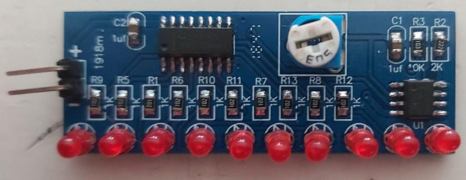
\includegraphics[width=0.8\linewidth]{P1/img/HasilSMD.png}
    \caption{Hasil SMD}
    \label{fig:HasilSMD}
\end{figure}
	\chapter{Dasar Desain Schematic dan PCB}

\section{Tujuan}
\begin{enumerate}
    \item Belajar mendesain sirkuit elektronik menggunakan software
    \item Mengetahui fungsi setiap komponen dan cara implementasinya
    \item Memahami proses menyusun komponen agar bisa digunakan bersamaan dengan komponen lain untuk melakukan fungsi tertentu
    \item Untuk memperkenalkan beberapa konsep dasar dan teknik laboratorium dalam mendesain schematic dan PCB
    \item Mendesain rangkaian PCB yang nantinya dapat dicetak menjadi komponen dengan fungsi tertentu
\end{enumerate}


\section{Dasar Teori}
Sebelum menyusun hardware dan komponen kecil seperti IC di breadboard dan
bahkan mensoldernya di PCB, ada baiknya kita melakukannya di software terlebih dahulu agar
kita bisa mengecek kompatibilitas tiap komponen dan mengecekknya secara virtual
disamping secara rinci mengetahui fungsi setiap komponen yang hendak kita gunakan
nantinya. Pada praktikum kali ini akan digunakan software Fusion360 untuk mendesain
schematic dan PCB yang nantinya akan diprint, selain memiliki fitur yang mumpuni, banyak
tutorial cara penggunaan serta tersedia banyak library komponen yang sering kali dipakai
pada project arduino, MCU, dan elektronika.

Praktikan diharapkan sudah membaca secara rinci modul instalasi Fusion360 dan mencoba fitur-fitur dasarnya dengan membuat schematic sederhana. Pada kali ini praktikan
akan arahkan untuk membuat rangkaian schematic dan board menggunakan MCU ESP-8266
dan beberapa komponen lain yang bisa diprogram menjadi alat IoT sederhana.

Kesalahan yang seringkali dijumpai pada proses desain PCB yaitu routing yang
membingunkan bagi pemula, atau jika sudah melakukan routing namun desainnya sulit
dipahami oleh pengguna lain, maka dari itu untuk memudahkan pembacaan schematic
digunakanlah fitur name dan label, hal ini digunakan untuk menyederhanakan desain tanpa
mengurangi sedikitpun fungsi utama sirkuit tersebut. Untuk mengecek apakah komponen
tersebut telah terkoneksi, gunakan fitur SHOW dan arahkan kursor mouse ke arah kabel yang
ingin dicek, dan jika kabel pada ujung dan pangkal sama-sama ter-highlight maka komponen
yang mendapat suplai daya tersebut sudah pasti terkoneksi dengan benar.

\section{Tugas Pendahuluan}
\begin{enumerate}
    \item Buatlah Wiring Schematic Minimum System ESP8266! Caranya seperti dibawah.
\end{enumerate}

\section{Wiring Schematic Minimum System ESP8266}
Untuk Tugas Pendahuluan, akan dibuat sebuah desain schematic Minimum System untuk menjalankan 
chip ESP8266 sehingga dapat dihubungkan dengan komputer dan dilakukan flash program ke ROM nya. 
Minimum System ESP8266 ini akan disuply dayanya dengan tegangan sebesar 3,3 Volt yang diatur 
oleh 3,3-Voltage Regulator nya. Untuk dapat menyambungkan ESP8266 dengan host computer yang 
dapat melakukan flash programnya maka digunakan connector TYPE-C 16Pin, 
sebagai penghubung koneksi ESP8266 dengan host computer. Selain itu, juga bisa menggunakan JST 4Pin TTL to USB.
Minimum System dari ESP8266 juga memiliki 
2 switch yang digunakan untuk melakukan Reset dan Flash.
\begin{enumerate}
    \item Untuk memulai membuat project klik \textbf{New Project} di kiri atas dan beri nama sesuai yang kalian inginkan
        \begin{figure}[H]
            \centering
            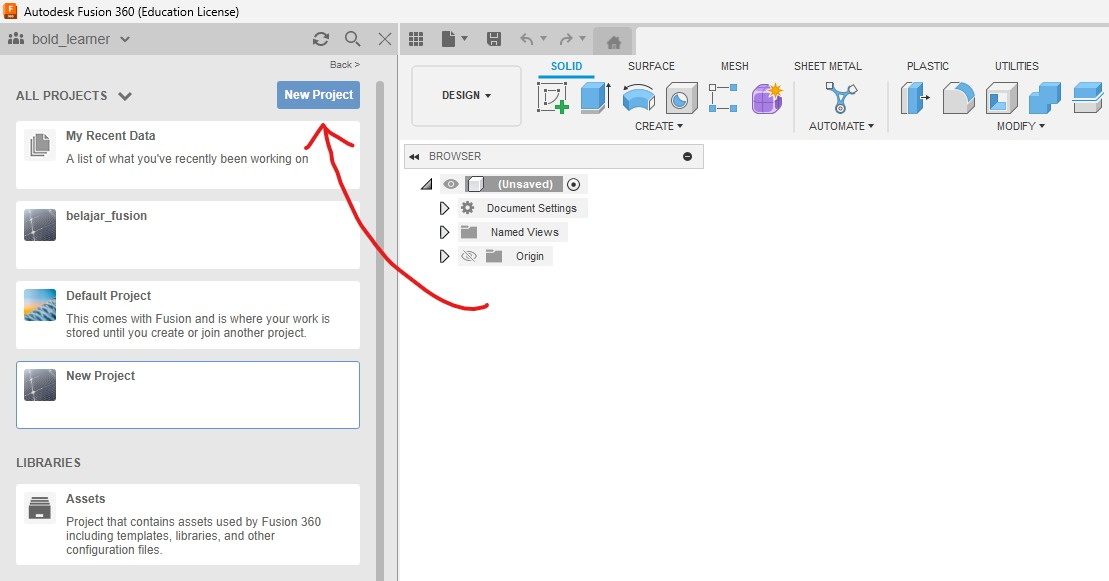
\includegraphics[width=0.6\linewidth]{P2/img/gambar1.jpeg}
            \caption{buat project baru} 
            \label{fig:buat project baru}
        \end{figure}
    \item Selanjut nya buka project space yang telah kalian buat pada window di bagian kiri
        \begin{figure}[H]
            \centering
            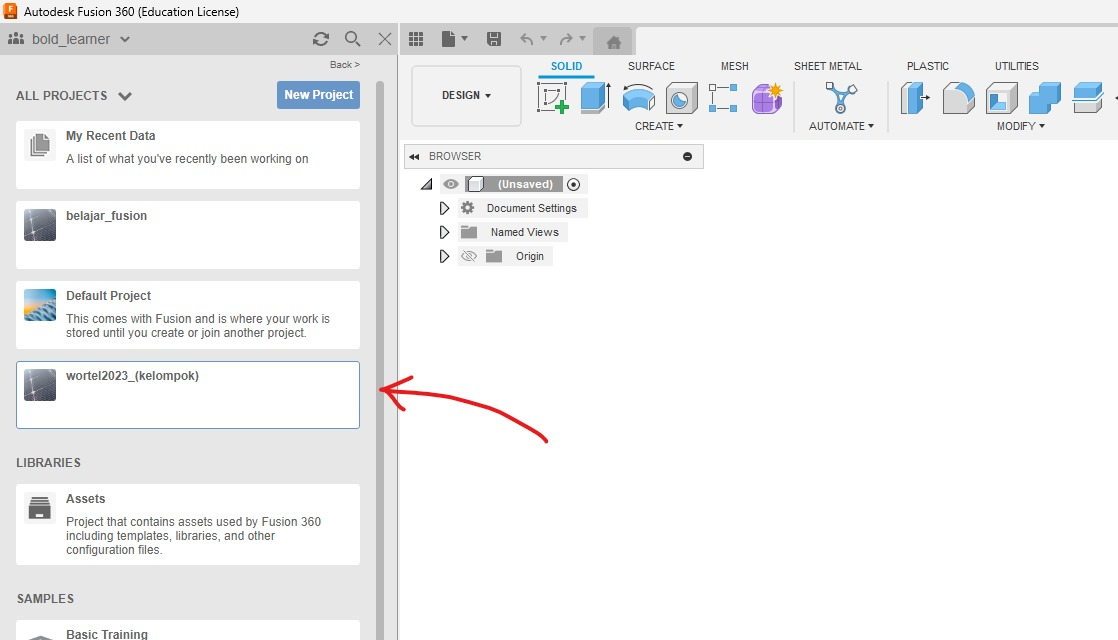
\includegraphics[width=0.6\linewidth]{P2/img/gambar2.jpeg}
            \caption{buka project} 
            \label{fig:buka project}
        \end{figure}
    \item Sebelum memulai mengerjakan pada project, kita harus mengimport library yang berisi semua komponen yang diperlukan. Klik \textbf{File > Open}
        \begin{figure}[H]
            \centering
            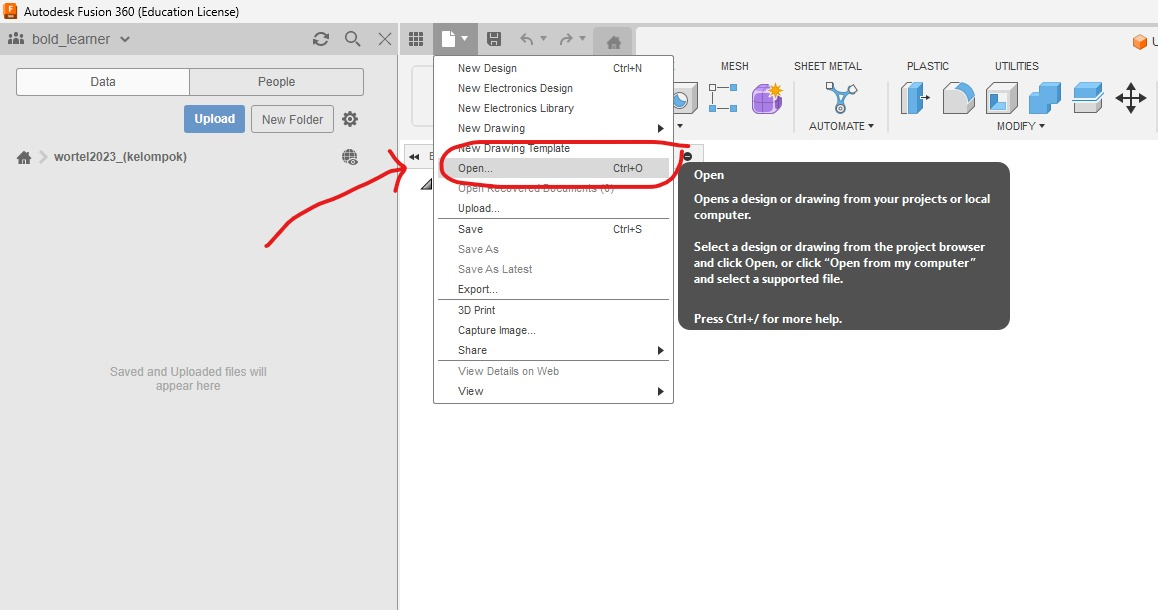
\includegraphics[width=0.6\linewidth]{P2/img/gambar3.jpeg}
            \caption{Membuka prompt File Select} 
            \label{fig:Membuka prompt File Select}
        \end{figure}
    Selanjutnya pilih \textbf{Open from my computer}
    \begin{figure}[H]
        \centering
        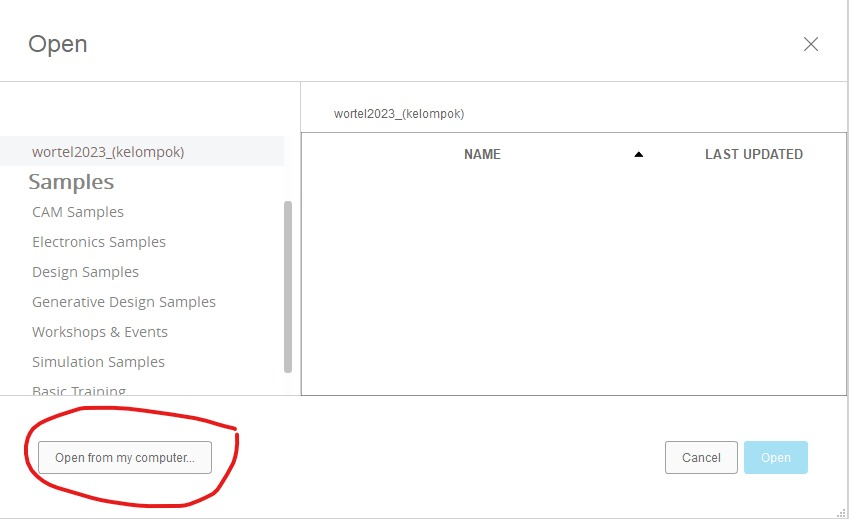
\includegraphics[width=0.6\linewidth]{P2/img/gambar4.jpeg}
        \caption{Mengakses file di Komputer} 
        \label{fig:Mengakses file di Komputer}
    \end{figure}
    Cari dimana file library untuk modul ini tersimpan pada folder file anda, file tersebut memiliki extensi file .lbr
    \begin{figure}[H]
        \centering
        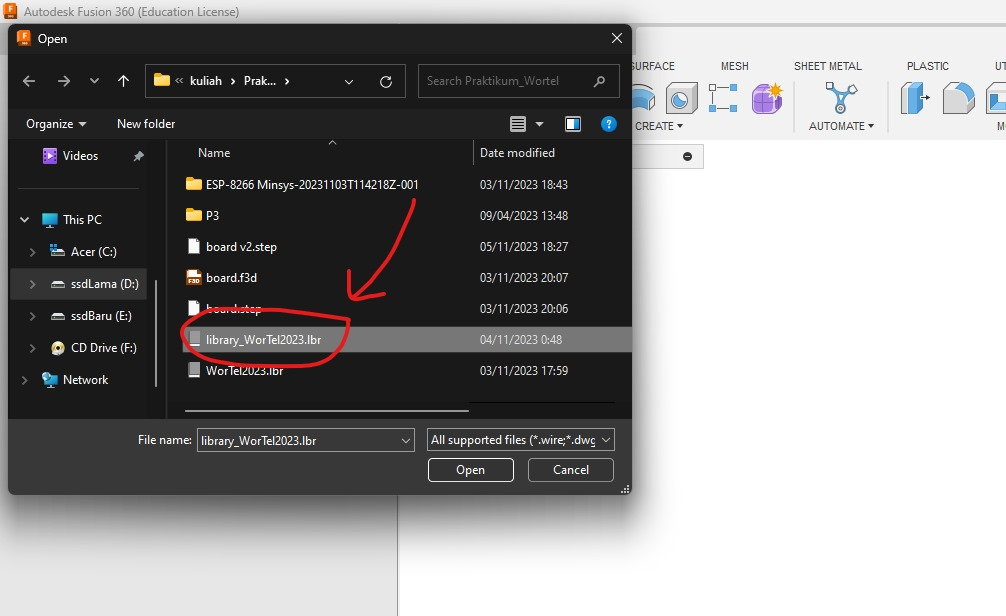
\includegraphics[width=0.6\linewidth]{P2/img/gambar5.jpeg}
        \caption{Memilih Library} 
        \label{fig:Memilih Library}
    \end{figure}
    Setelah library terimport, klik \textbf{ctrl + S} untuk melakukan saving library pada project yang anda miliki dan klik save.
    \begin{figure}[H]
        \centering
        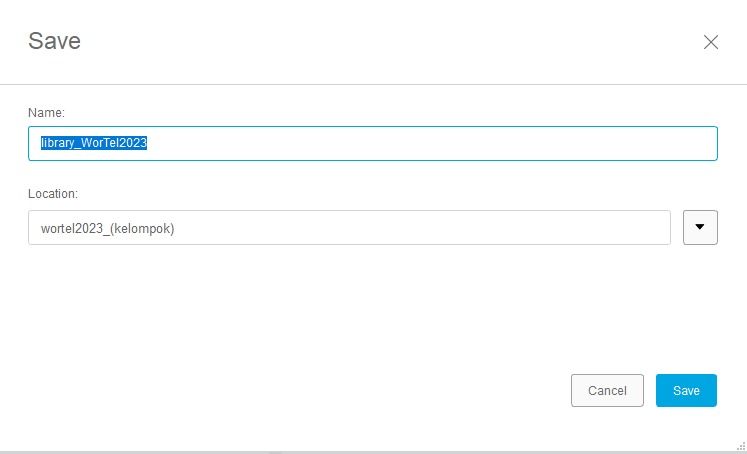
\includegraphics[width=0.6\linewidth]{P2/img/gambar6.jpeg}
        \caption{Simpan Library} 
        \label{fig:Simpan Library}
    \end{figure}
    Maka tampilan Fusion anda akan menjadi seperti \textbf{Gambar 1.7}, dimana telah terdapat list komponen yang anda perlukan.
        \begin{figure}[H]
            \centering
            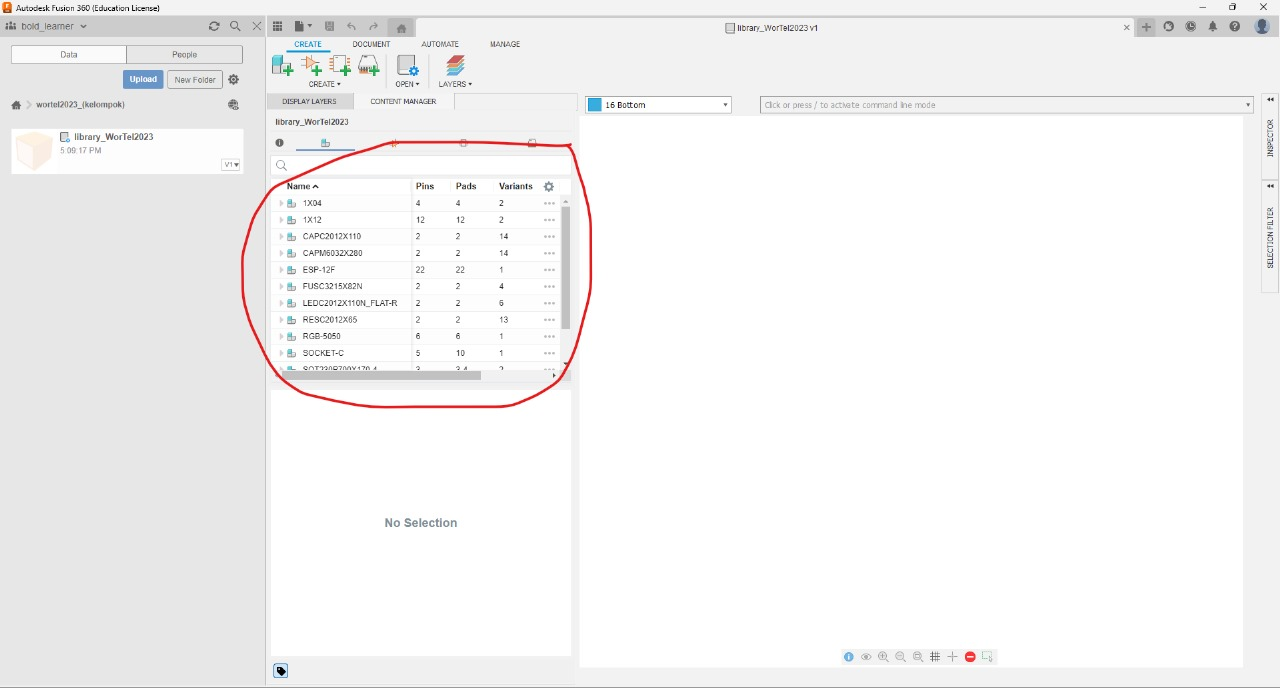
\includegraphics[width=0.6\linewidth]{P2/img/gambar7.jpeg}
            \caption{Tampilan Fusion} 
            \label{fig:TampilanFusion1}
        \end{figure}
    \item Berikutnya untuk memulai mendesign rangkaian, klik \textbf{File > New Electonic Design}
        \begin{figure}[H]
            \centering
            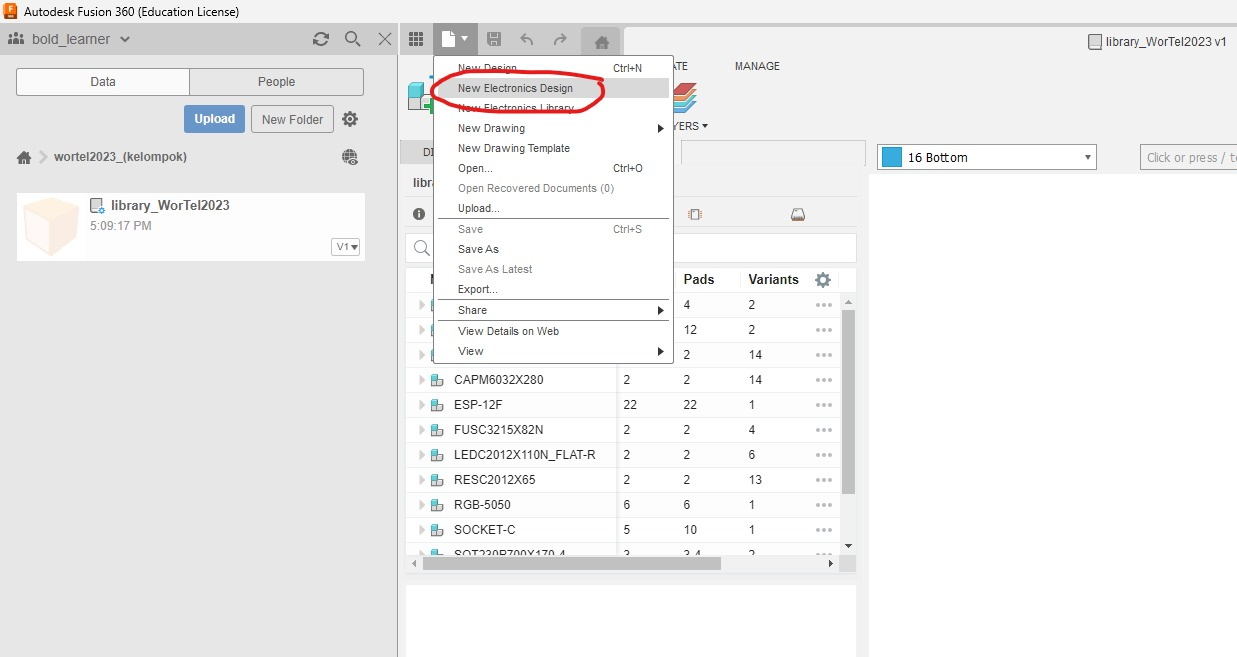
\includegraphics[width=0.6\linewidth]{P2/img/gambar8.jpeg}
            \caption{Memulai desain rangkaian} 
            \label{fig:Memulai desain rangkaian}
        \end{figure}
    Lakukan penyimpanan dengan menekan \textbf{ctrl + S} lalu beri nama sesuai keinginan kalian.
        \begin{figure}[H]
            \centering
            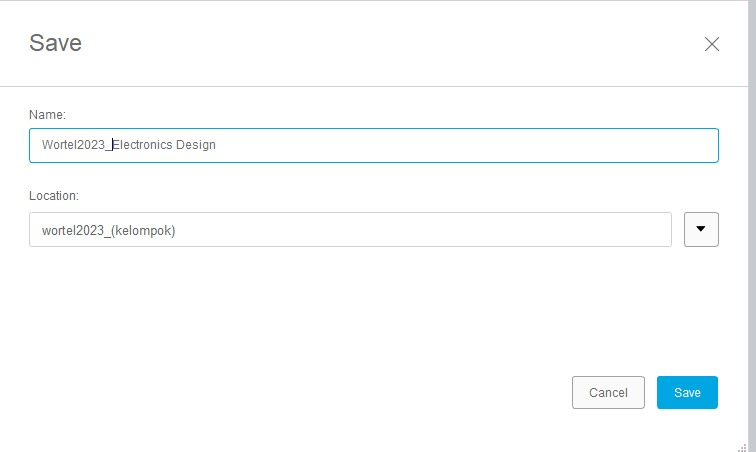
\includegraphics[width=0.6\linewidth]{P2/img/gambar9.jpeg}
            \caption{Menyimpan workspace} 
            \label{fig:Menyimpan workspace}
        \end{figure}
    Tampilan Fusion anda akan menjadi seperti \textbf{gambar 1.10}
        \begin{figure}[H]
            \centering
            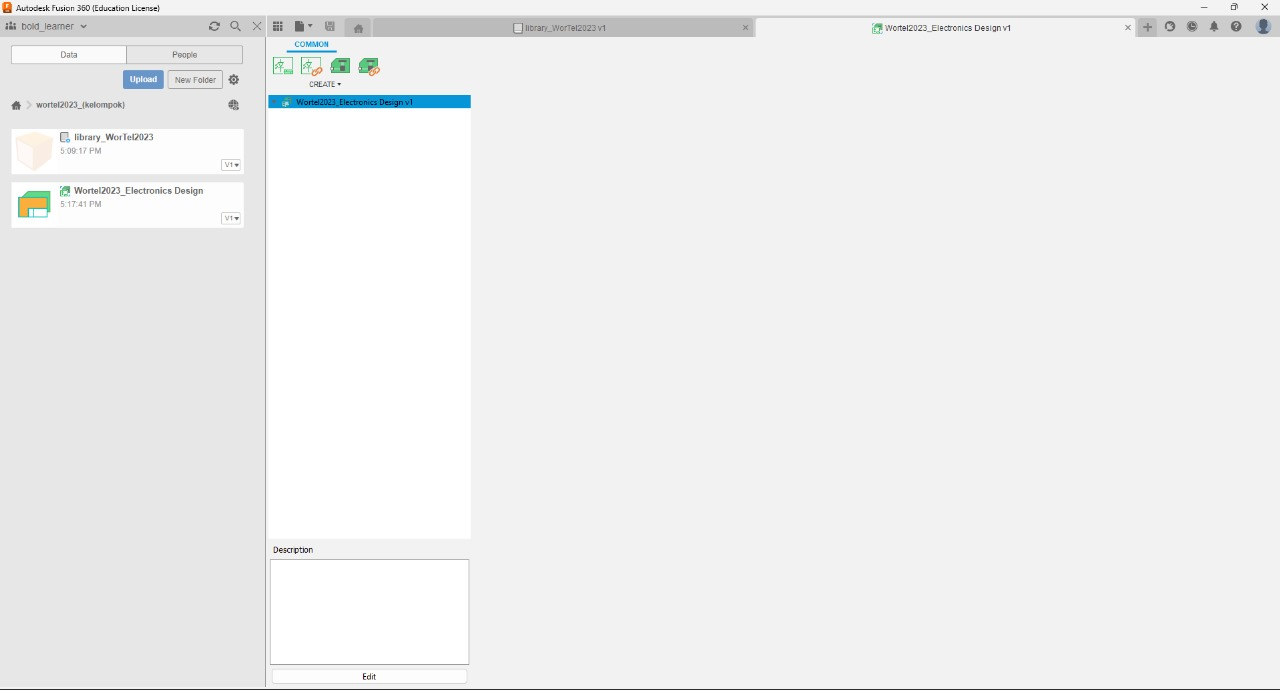
\includegraphics[width=0.6\linewidth]{P2/img/gambar10.jpeg}
            \caption{Tampilan Fusion} 
            \label{fig:Tampilan Fusion}
        \end{figure}
    \item Untuk membuat lembar schematic dan mulai mendesain, klik tombol \textbf{New Schematic} 
        \begin{figure}[H]
            \centering
            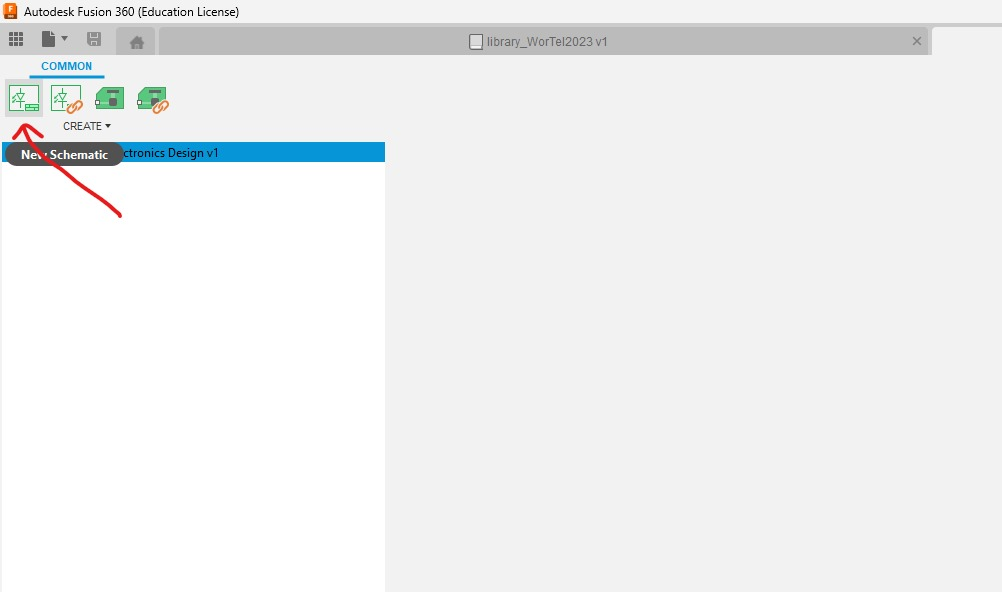
\includegraphics[width=0.6\linewidth]{P2/img/gambar11.jpeg}
            \caption{New Schmatic} 
            \label{fig:New Schematic}
        \end{figure}
    berikutnya tekan \textbf{ctrl + S} lalu beri nama dan simpan schematic.
    \item Untuk meletakan komponen, dapat menggunakan tool \textbf{Place Component} yang terletak pada bagian dari Fusion.
        \begin{figure}[H]
            \centering
            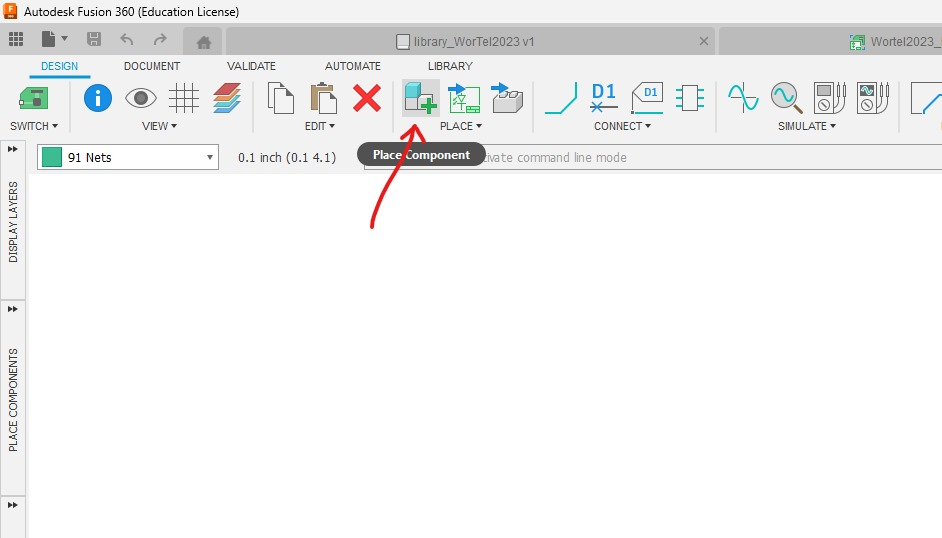
\includegraphics[width=0.6\linewidth]{P2/img/gambar13.jpeg}
            \caption{Place Component} 
            \label{fig:Place Component}
        \end{figure}
    \item Tekan icon \textbf{Open Library Manager} sesuai dengan \textbf{gambar 1.14}
        \begin{figure}[H]
            \centering
            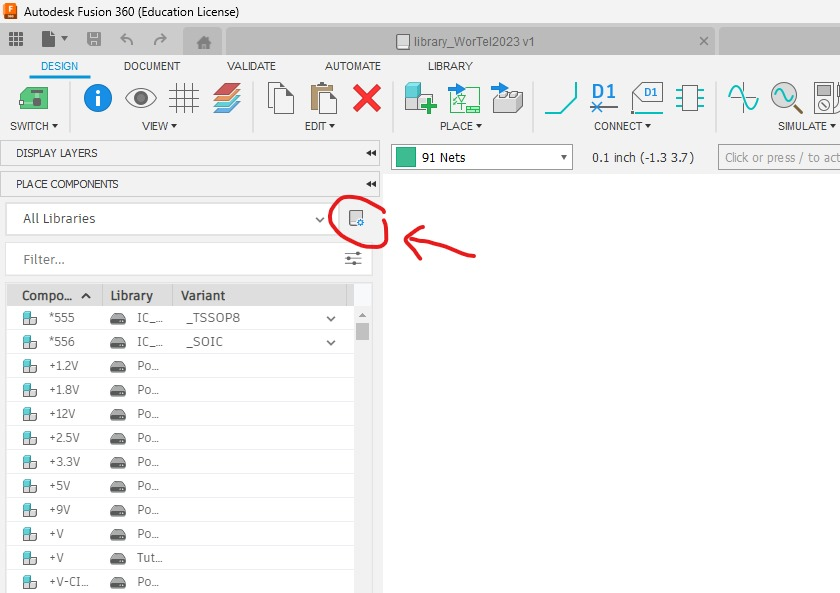
\includegraphics[width=0.6\linewidth]{P2/img/gambar14.jpeg}
            \caption{Membuka Library Manager} 
            \label{fig:Membuka LIbrary Manager}
        \end{figure}
    Berikutnya aktifkan library yang sebelumnya telah anda tambahkan dan pastikan statusnya \textbf{In Use}
        \begin{figure}[H]
            \centering
            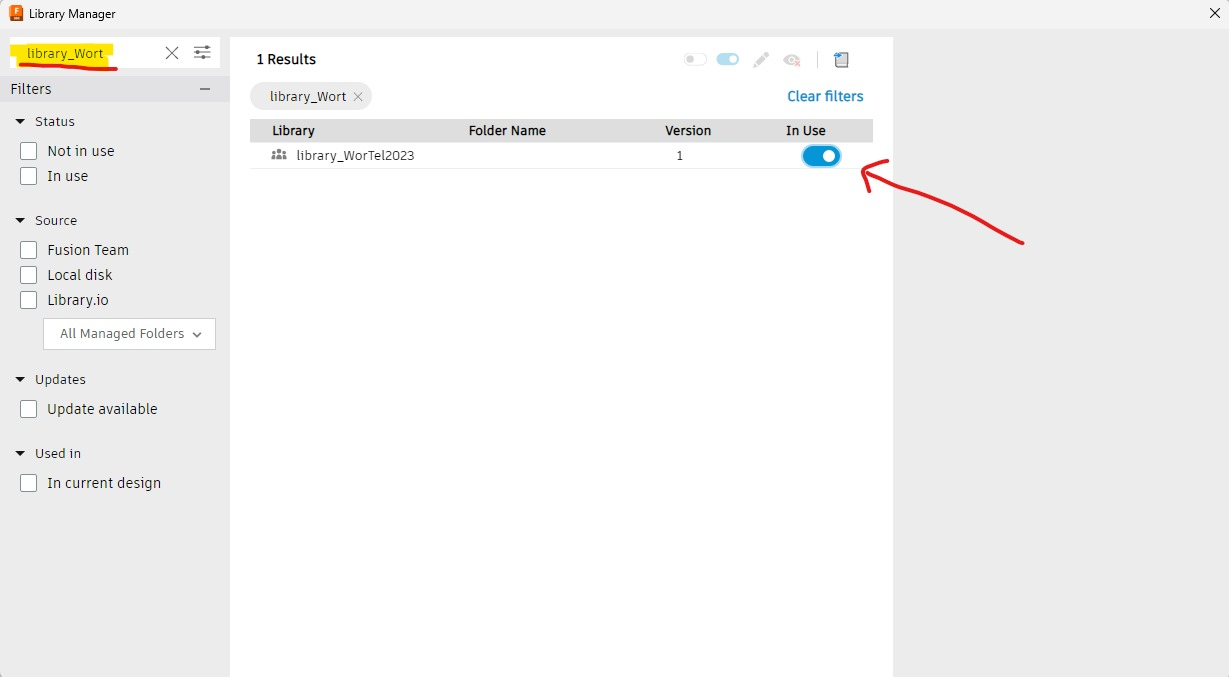
\includegraphics[width=0.6\linewidth]{P2/img/gambar15.jpeg}
            
            
            \label{fig:Status Library}
        \end{figure}

    \newpage
    \item Berikut adalah komponen-komponen yang anda butuhkan :
    \vspace{5pt}
    \begin{table}[ht]
        
   
    \begin{center}
    
        \caption{Komponen}
        \label{tab:komponen}

        \begin{tabular}{|c|p{2cm}|m{2cm}|m{2cm}|m{2cm}|}
            \hline
            Gambar & Nama & Library & Jumlah & Catatan \\
            \hline
            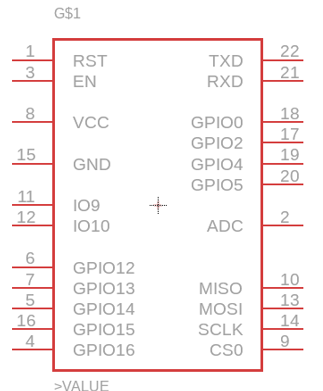
\includegraphics[width=0.05\linewidth]{P2/img/ESP-12F_2.png} & {\fontsize{8}{6}\selectfont ESP-12F} & {\fontsize{8}{6}\selectfont WorTel Library} & 1 &  - \\
            \hline
            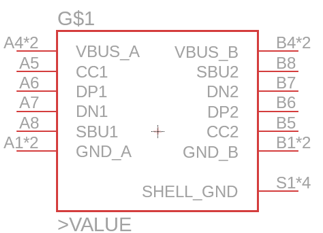
\includegraphics[width=0.05\linewidth]{P2/img/USB-C_2.png} & {\fontsize{8}{6}\selectfont USB-C} &  {\fontsize{8}{6}\selectfont WorTel Library} & 1 & - \\
            \hline
            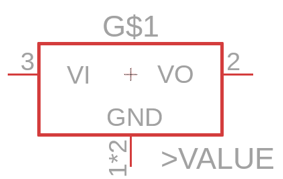
\includegraphics[width=0.05\linewidth]{P2/img/Regulator_3V3_2.png} & {\fontsize{8}{6}\selectfont Regulator 3V3} &  {\fontsize{8}{6}\selectfont WorTel Library} & 1 & - \\
            \hline
            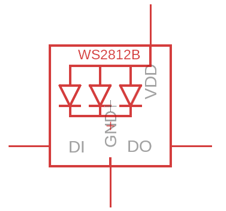
\includegraphics[width=0.1\linewidth]{P2/img/WS2812B_2.png} & {\fontsize{8}{6}\selectfont WS2812B} &  {\fontsize{8}{6}\selectfont WorTel Library} & 1 & - \\
            \hline
            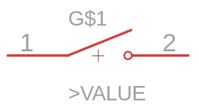
\includegraphics[width=0.1\linewidth]{P2/img/Button_2.png} & {\fontsize{8}{6}\selectfont Button} &  {\fontsize{8}{6}\selectfont WorTel Library} & 2 & - \\
            \hline
            
\includegraphics[width=0.1\linewidth]{P2/img/Capacitor_2.png} & {\fontsize{8}{6}\selectfont Capacitor} &  {\fontsize{8}{6}\selectfont WorTel Library} & 3 & {\fontsize{8}{6}\selectfont 100uF(1), 10uF(2)} \\
            \hline
            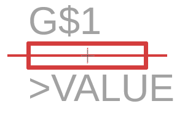
\includegraphics[width=0.1\linewidth]{P2/img/Fuse_2.png} & {\fontsize{8}{6}\selectfont Fuse} &  {\fontsize{8}{6}\selectfont WorTel Library} & 1 & - \\
            \hline
            
\includegraphics[width=0.1\linewidth]{P2/img/LED_2.png} & {\fontsize{8}{6}\selectfont LED} &  {\fontsize{8}{6}\selectfont WorTel Library} & 1 & - \\
            \hline
            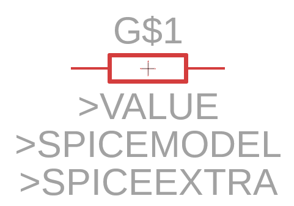
\includegraphics[width=0.1\linewidth]{P2/img/RESISTOR_2.png} & {\fontsize{8}{6}\selectfont Resistor} &  {\fontsize{8}{6}\selectfont WorTel Library} & 7 & {\fontsize{8}{6}\selectfont 10k(4), 5.1k(2), 1k(1)} \\
            \hline
            \end{tabular}
        \vspace{-\topsep} % Mengurangi spasi sebelum tabel
    \end{center}
\end{table}
    \vspace{5pt}
    \\
    \\
    \item Sambungkan seluruh komponen dengan koneksi pin.
    \item Hasil dari rangkaian dari Minimum System ESP8266 adalah sebagai berikut :
        \begin{figure}[H]
            \centering
            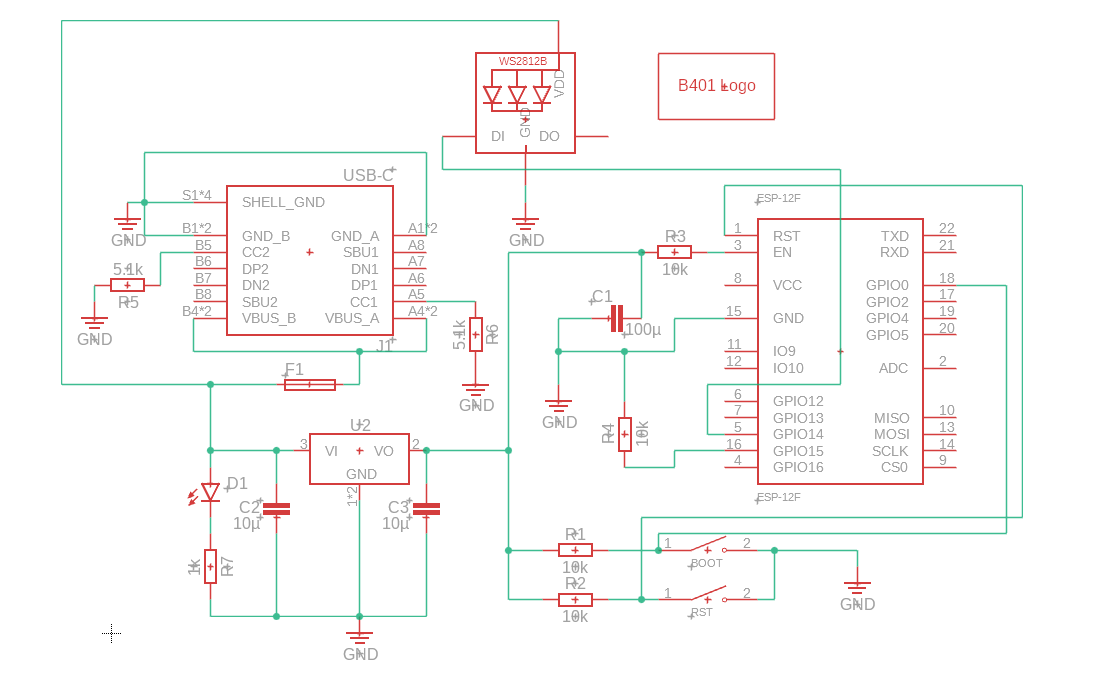
\includegraphics[width=0.6\linewidth]{P2/img/Hasil Schematic .png}
            \caption{Hasil Rangkaian} 
            \label{fig:Hasil Rangkaian}
        \end{figure}
\end{enumerate}
\newpage

\section{Alat dan Komponen}
\subsection{Alat}
\begin{enumerate}
    \item Laptop yang telah terinstall Autodesk Fusion 360
    \item Mouse
\end{enumerate}

\section{Eksperimen 1: PCB design Minimum System ESP8266}
Setelah proses penyusunan schematic selesai, waktunya mendesain bagaimana Printed Circuit Board
dari schematic tersebut akan tersusun.
\begin{enumerate}
    \item Untuk melanjutkan mendesain board dari schematic gunakan tools \textbf{“Switch to PCB
    documentation”}
    \begin{figure}[H]
        \centering
        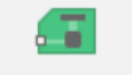
\includegraphics[width=0.4\linewidth]{P2/img/switchtopcb.png}
        \caption{Switch to PCB} 
        \label{fig:Switch to PCB}
    \end{figure}
    Pada bagian awal saat mengubah ke board, akan disuguhkan tampilan sebagai berikut. Pada
    bagian kiri terdapat Footprint dari komponen dengan garis warna kuning yang
    menghubungkan antar footprint komponen sesuai dengan wiring pada schematic. Pada
    bagian kanan terdapat “Board” yang berbentuk persegi hitam yaitu tempat untuk meletakan
    footprint komponen.
    \begin{figure}[H]
        \centering
        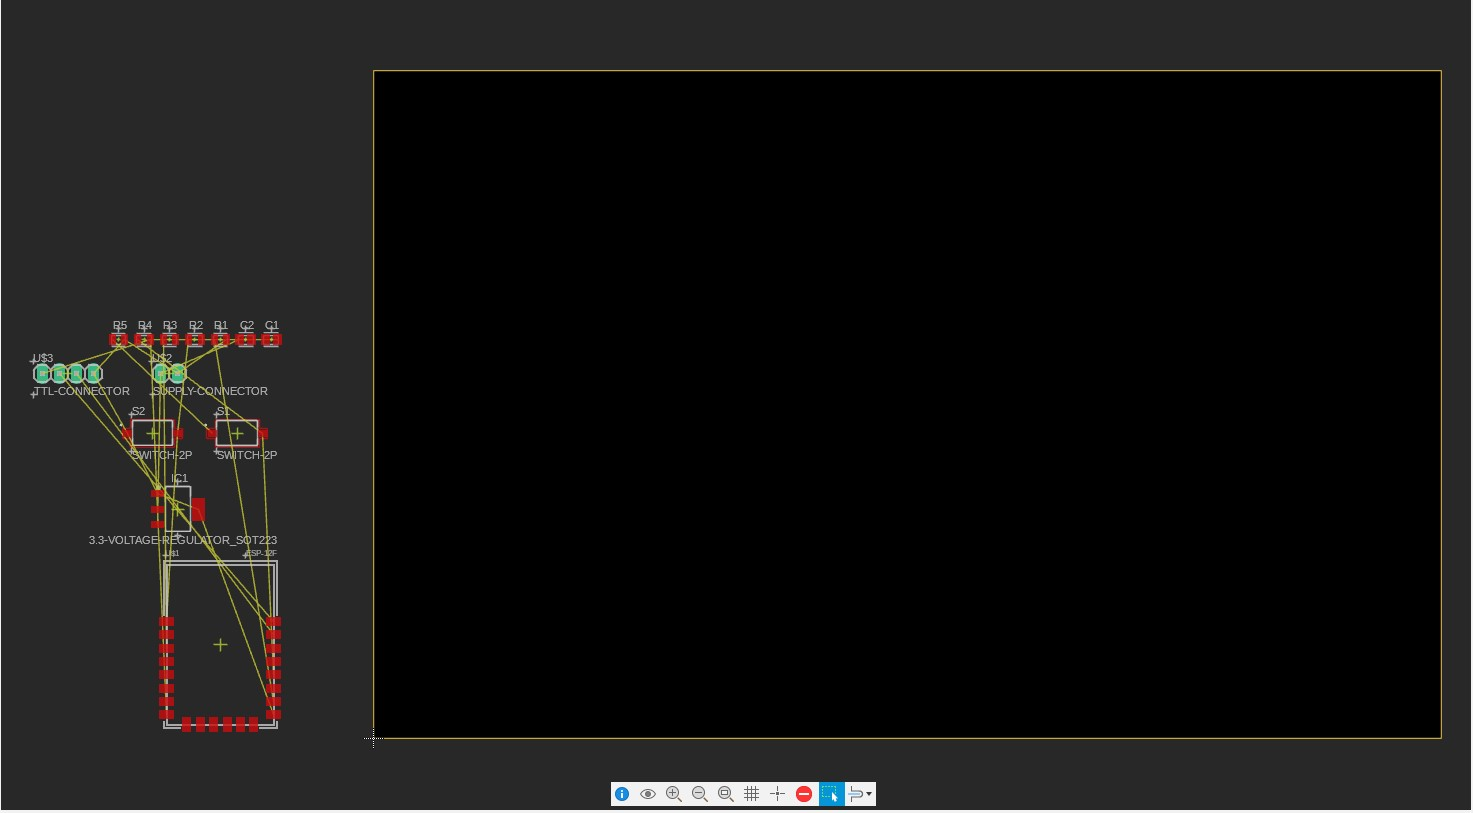
\includegraphics[width=0.6\linewidth]{P2/img/awal_switch_ke_pcb_design.jpg}
        \caption{PCB awal} 
        \label{fig:PCBawal}
    \end{figure}
    \vspace{-\topsep}
    \item Masukan seluruh footprint komponen ke dalam Board dengan memilih seluruh footprint menggunakan tools \textbf{Group} dan digerakan dengan menggukan tools \textbf{Move}.
    \begin{figure}[H]
        \centering
        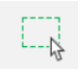
\includegraphics[width=0.15\linewidth]{P2/img/group.png}
        
\includegraphics[width=0.12\linewidth]{P2/img/move.png}
        \caption{Group dan Move}
    \end{figure}
    \begin{figure}[H]
        \centering
        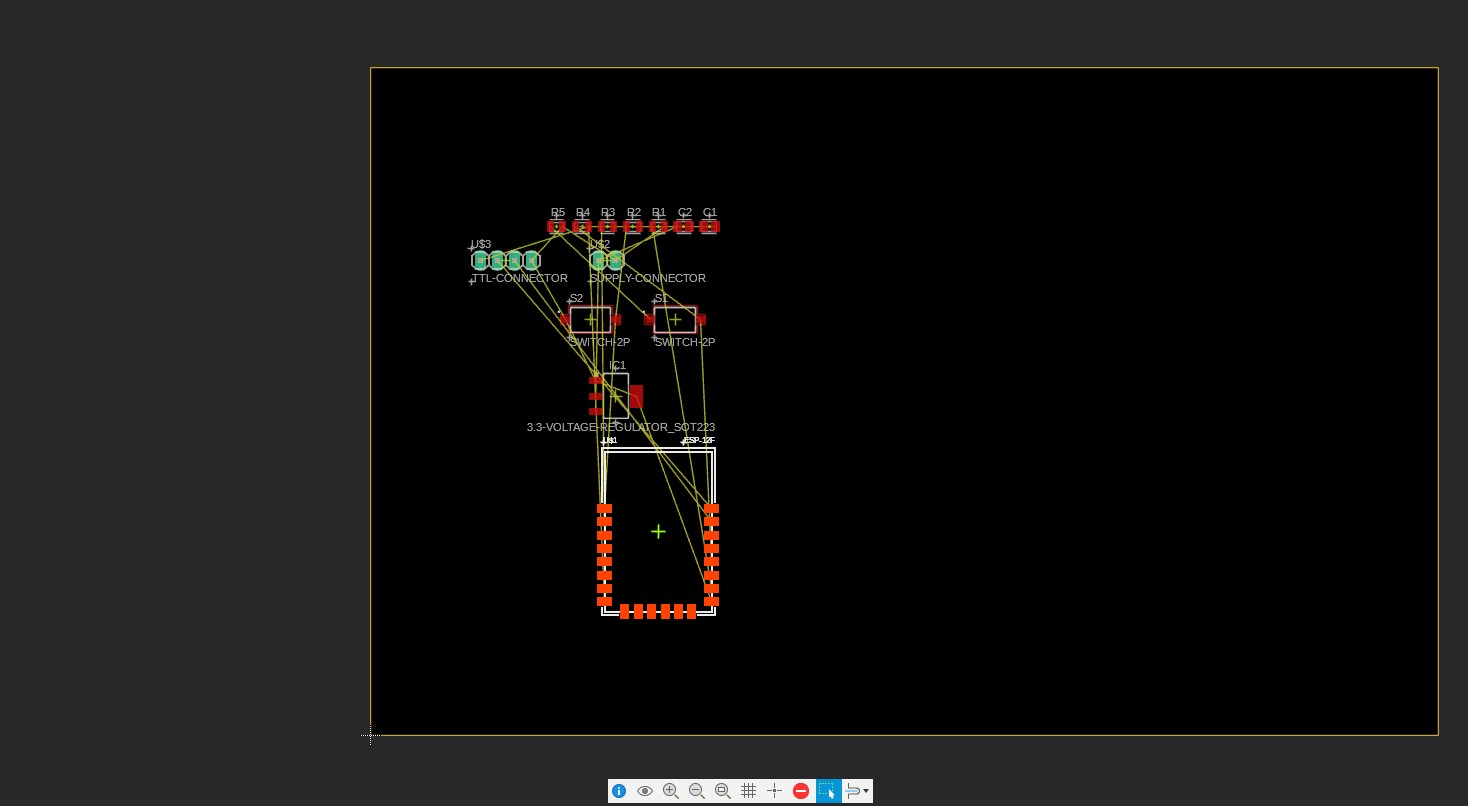
\includegraphics[width=0.6\linewidth]{P2/img/masukkan_semua_komponen_ke_lingkup_pcb.jpg}
        \caption{Hasil setelah dipindah} 
        \label{fig:Hasil setelah dipindah}
    \end{figure}
    \item Susun footprint serapi mungkin dengan mengerakan footprint menggunakan tools
    \textbf{Move}
        \begin{figure}[H]
            \centering
            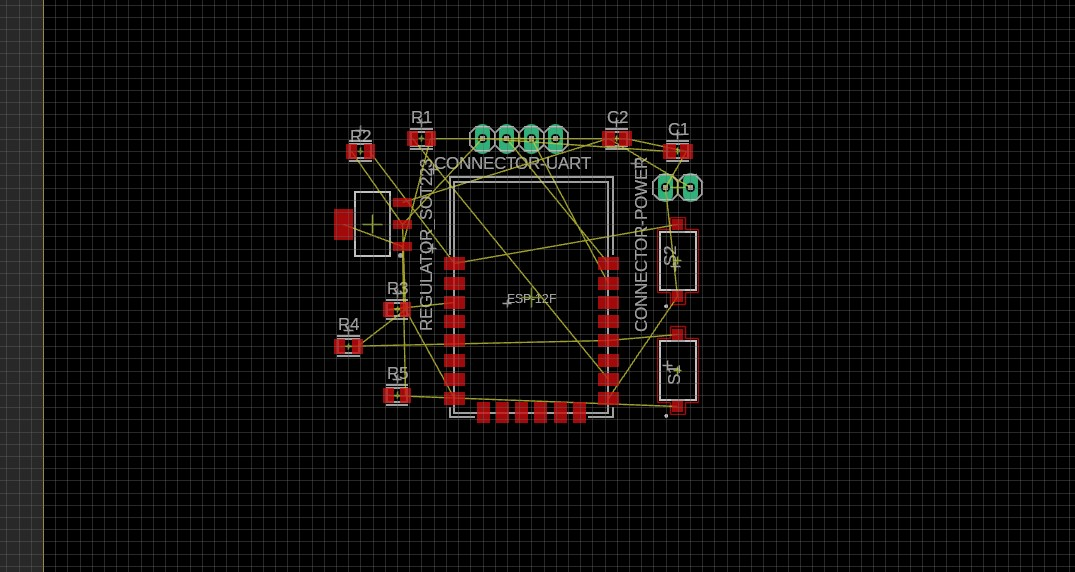
\includegraphics[width=0.6\linewidth]{P2/img/rapihkan_tatanan_komponen.jpg}
            \caption{PCB awal} 
            \label{fig:PCB awal}
        \end{figure}
    \item Raphikan tatanan komponen serta atur ukuran “Board” dengan menggerakan/geser garis tepi dari “Board” hingga ukuran
    sesuai dengan tatanan footprint.
        \begin{figure}[H]
            \centering
            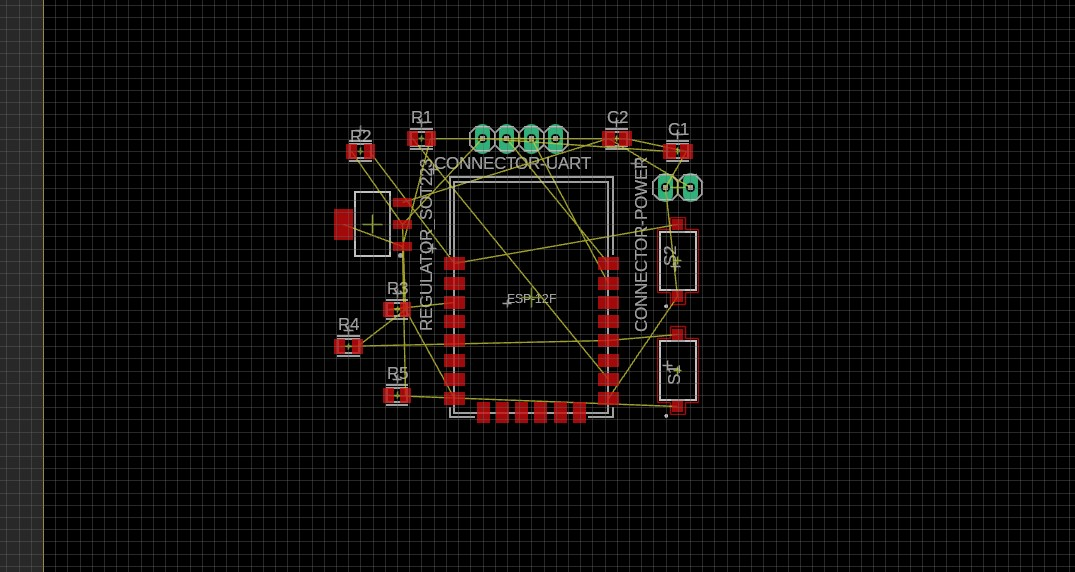
\includegraphics[width=0.5\linewidth]{P2/img/rapihkan_tatanan_komponen.jpg}
            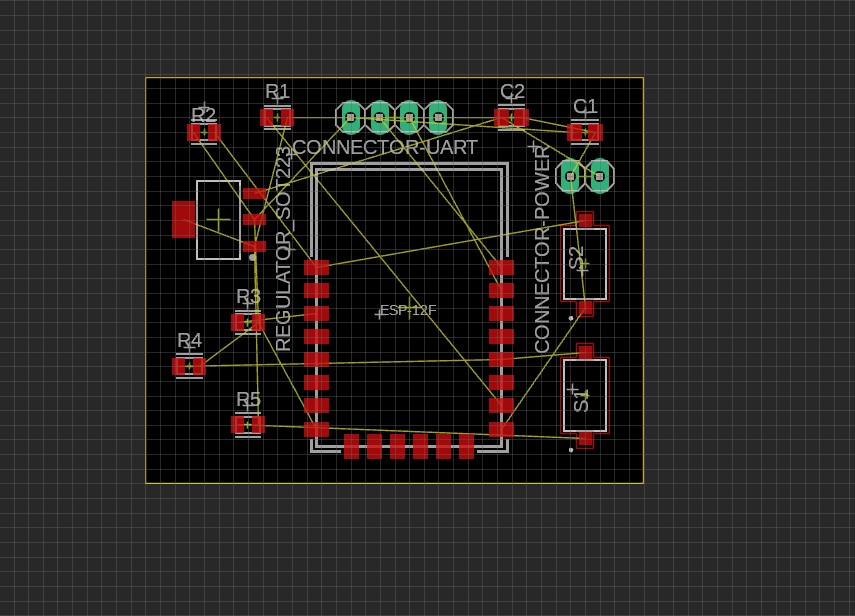
\includegraphics[width=0.45\linewidth]{P2/img/hasil_rapi.jpg}
            \caption{Setelah board dikecilkan} 
            \label{fig:Setelah komponen dirapihkan dan dikecilkan}
        \end{figure}
    \item Selanjutnya adalah melakukan routing jalur koneksi. Dalam melakukan Routing, Tools
    utama yang digunakan adalah \textbf{Route Manual} dan \textbf{Unroute} untuk
    menghapus route. Jalur Routing mengikuti garis warna kuning.
        \begin{figure}[H]
            \centering
            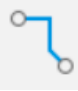
\includegraphics[width=0.12\linewidth]{P2/img/manualroute.png}
            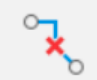
\includegraphics[width=0.17\linewidth]{P2/img/unroute.png}
            \caption{Manual route dan unroute}
        \end{figure}
        \begin{figure}[H]
            \centering
            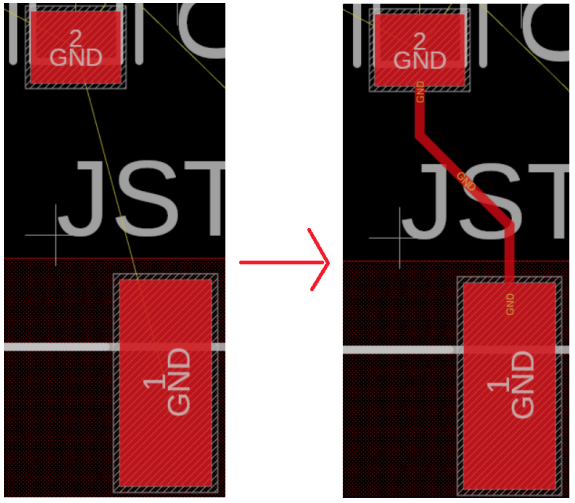
\includegraphics[width=0.89\linewidth]{P2/img/routing1.png}
            \caption{Contoh cara routing}
        \end{figure}
    \item Saat menggunakan Routing normalnya layer yang digunakan adalah \textbf{1 Top} akan tetapi
    Routing yang dibuat di layer yang sama tidak bisa saling ditabrak/ tumpuk.
        \begin{figure}[H]
            \centering
            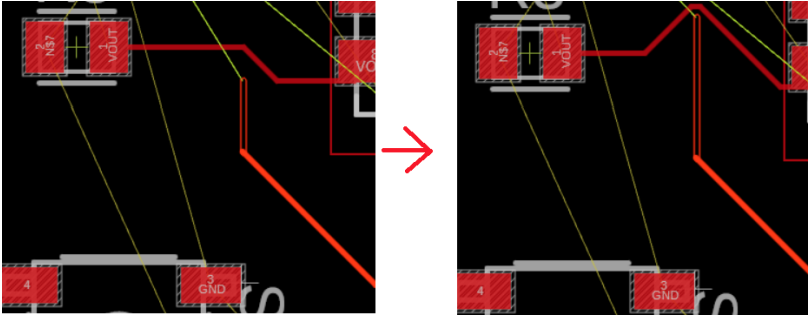
\includegraphics[width=0.89\linewidth]{P2/img/routing2.png}
            \caption{Contoh routing routing yang bertabrakan}
        \end{figure}
    Maka untuk mengatasi hal itu dapat digunakan layer yang lain. Untuk berpindah layer
    menjadi \textbf{16 Bottom} saat menggunakan Route Manual dapat di klik mouse 3 (scroll wheel)
    untuk meletakan \textbf{Vias} yaitu lingkaran penghubung layer top dan bottom. Berpindah layer
    berfungsi agar jalur routing tidak bertabrakan.
        \begin{figure}[H]
            \centering
            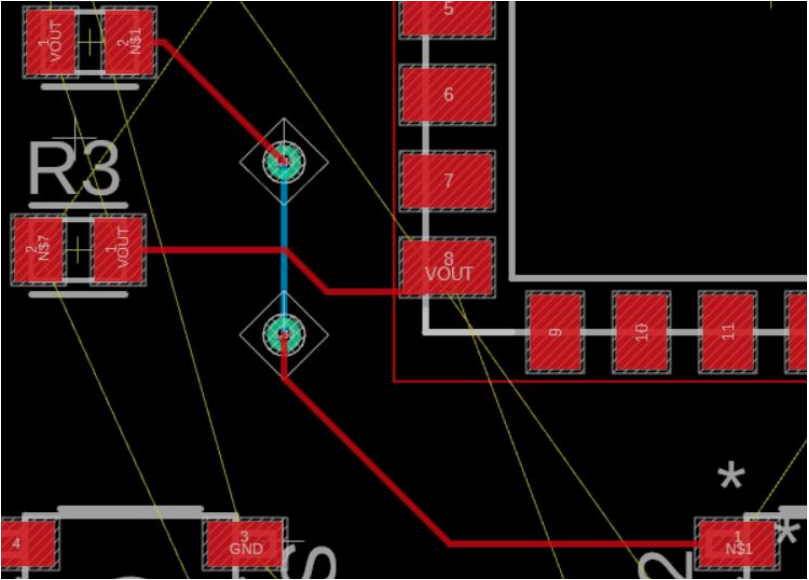
\includegraphics[width=0.89\linewidth]{P2/img/routing3.png}
            \caption{Vias yang menghubungkan Routing top(merah) dengan Bottom(biru)}
        \end{figure}
    \item Routing Seluruh garis koneksi warna kuning hingga seluruhnya tersambung. \textbf{
    Pastikan jalur Routing tidak saling berdekatan dengan jalur lain.}
        \begin{figure}[H]
            \centering
            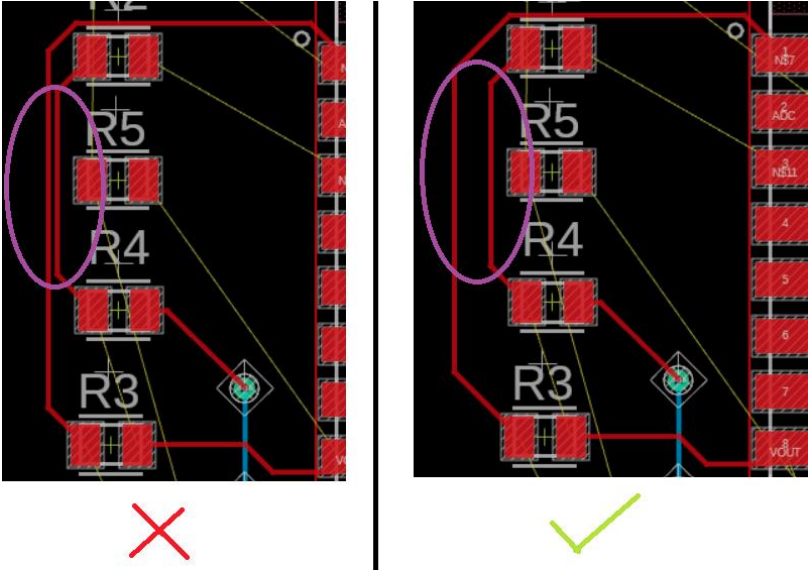
\includegraphics[width=0.89\linewidth]{P2/img/routing4.png}
            \caption{Contoh rangkaian yang tidak bagus dan bagus}
        \end{figure}

    \item Setelah selesai klik save (ctrl+s).
    \textbf{Contoh rangkaian PCB yang sudah jadi :}
        \begin{figure}[H]
            \centering
            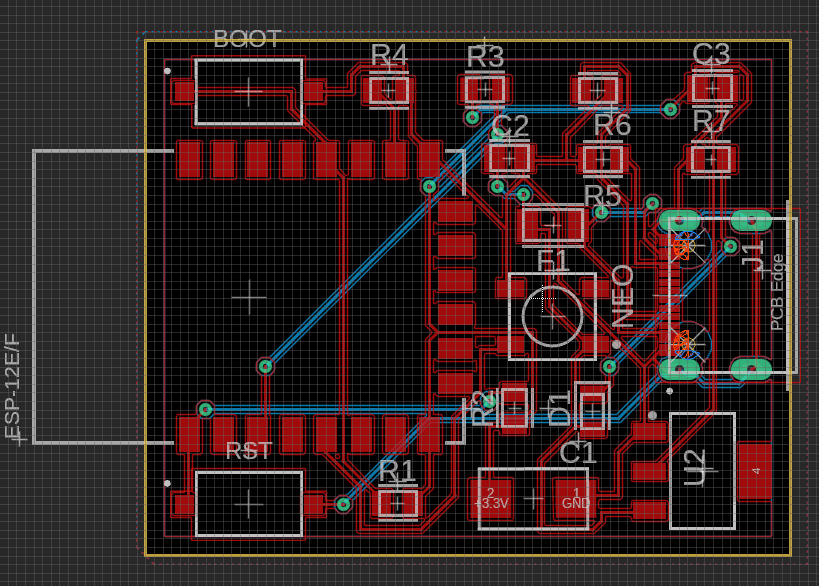
\includegraphics[width=0.47\linewidth]{P2/img/gambar_jadi.jpg}
            \caption{Hasil sesudah di routing}
        \end{figure}
\end{enumerate}
  \chapter{Dasar Desain 3D Model Fusion 360}

\section{Tujuan}
\begin{enumerate}
    \item Belajar mendesain model 3D menggunakan software
    \item Mengetahui berbagai tools yang tersedia pada software desain 3D serta fungsinya
    \item Mengetahui bagaimana melakukan slicing model 3D yang nantinya akan diprint
    \item Mengetahui bagaimana melakukan proses printing dengan 3D printer
\end{enumerate}

\section{Dasar Teori}
Secara sederhana, Enclosure adalah housing logam atau plastik yang dirancang untuk menutupi dan
melindungi disk drive, chip, ataupun board didalamnya dari kerusakan serta risiko lain yang bisa
membahayakan fungsionalitas dan keutuhan komponen didalamnya. Enclosure pada umumnya dapat
menampung satu board, dan memiliki ukuran yang pas dan sesuai, namun tetap memiliki lubang dan celah
sehingga board didalamnya masih bisa untuk dihubungkan ke komputer host.

Enclosure case yang efektif memungkinkan untuk ditaruh board dengan tepat, tidak sempit ataupun
longgar, mekanisme penutupan enclosure bisa menggunakan slide, mur, ataupun seperti lego sehingga
tetap tertutup meskipun digoyang dan digerakkan dengan gaya tertentu. Selain itu, enclosure ini
berfungsi untuk melindungi board dari hal-hal seperti kabel dengan tegangan tertentu yang dapat
membuat arus pendek pada board. Berikut referensi desain enclosure
\begin{figure}[H]
    \centering
    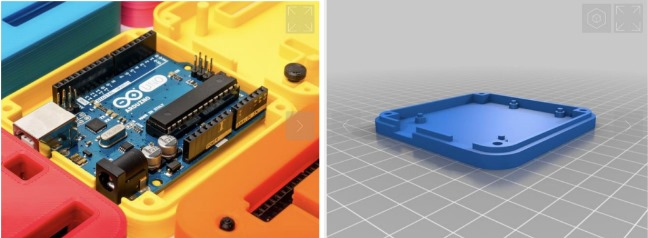
\includegraphics[width=1\linewidth]{P3/img/image1.jpg}
    \caption{Referensi Desain Enclosure}
    \label{fig:Referensi Desain Enclosure}
\end{figure}

\begin{figure}[H]
    \centering
    \includegraphics[width=1\linewidth]{P3/img/image2.jpg}
    \caption{Komponen Enclosure}
    \label{fig:Komponen Enclosure}
\end{figure}

Kesalahan yang seringkali dijumpai pada proses desain 3D yaitu alur kerja yang terlalu repetitive ataupun
bertele-tele, karena sebenarnya fitur software banyak yang kurang di-explore sehingga saat
menggunakan software, fitur yang digunakan kurang membantu pengerjaan desain atau bahkan
memperlamanya. Untuk itu hendaknya mencari referensi, dokumentasi, ataupun inspirasi yang terdapat
di sekitar seperti lego, laptop, ataupun projektil lain yang dapat ditiru, amati, dan modifikasi desainnya.

\section{Tugas Pendahuluan}
\begin{enumerate}
    \item Buat satu desain kubus pada fusion 360 seperti pada gambar dibawah ini
        \begin{figure}[H]
            \centering
            \includegraphics[width=0.25\linewidth]{P3/img/soal1.png}
            \caption{Tugas Pendahuluan}
            \label{fig:Tugas Pendahuluan}
        \end{figure}
    \item Install Ultimaker CURA
\end{enumerate}

\section{Alat dan Komponen}
\subsection{Alat}
\begin{enumerate}
    \item Laptop yang telah terinstall Autodesk Fusion 360
    \item Laptop yang telah terinstall Ultimaker CURA untuk print 3d
    \item Mouse
\end{enumerate}

\section{Eksperimen 1: Membuat Enclosure PCB}
Buatlah enclosure dari PCB yang disediakan. Enclosure harus terbagi setidaknya menjadi dua bagian yaitu
\textbf{“Bawah”} sebagai tumpuan PCB dan \textbf{“Atas”} sebagai penutup enclosure. Enclosure juga harus memiliki
lubang power untuk tempat memberi tegangan PCB.
\begin{enumerate}
    \item Sebelum mendesain, upload lah file model 3D dengan type file .stp yang sudah disediakan. Untuk
    mengupload model klik \textbf{“Upload”} di panel sebelah kiri.
        \begin{figure}[H]
            \centering
            \includegraphics[width=0.5\linewidth]{P3/img/image3.jpg}
            \caption{Upload}
            \label{fig:Upload}
        \end{figure}

    \item Untuk memulai mendesain Enclosure klik pada \textbf{“file”} dan klik pada \textbf{“New Design”} atau juga saat
    membuka fusion otomatis new design akan terbuka sendirinya. Setelah new design terbuka klik
    save (ctrl + s) dan beri nama terserah.
        \begin{figure}[H]
            \centering
            \includegraphics[width=0.5\linewidth]{P3/img/image4.jpg}
            \caption{New Design}
            \label{fig:New Design}
        \end{figure}

    \item Langkah selanjutnya adalah memasukan model PCB 3D yang sudah diupload sebelumnya. Untuk
    memasukan model PCB klik kanan pada model tersebut lalu klik \textbf{“Insert into current Design”}.
        \begin{figure}[H]
            \centering
            \includegraphics[width=0.5\linewidth]{P3/img/Insert to Current Design 2.jpg}
            \caption{Insert Into Curret Design}
            \label{fig:Insert Into Curret Design}
        \end{figure}

        \begin{figure}[H]
            \centering
            \includegraphics[width=0.5\linewidth]{P3/img/Insert PCB.jpg}
            \caption{Sudah di Insert}
            \label{fig:Sudah di Insert}
        \end{figure}

    \item Saat membuat enclosure terdapat beberapa tools yang tersedia. Berikut beberapa tools yang
    akan sering digunakan dalam pembuatan enclosure:
        \begin{figure}[H]
            \centering
            \includegraphics[width=0.1\linewidth]{P3/img/image6.jpg}
            \caption{Sketch}
            \label{fig:Sketch}
        \end{figure}
        
        \textbf{Sketch}: menggambar sketsa 2D dari bentuk yang akan dibuat. Sketsa ini dapat digunakan
        bersama Extrude untuk membuat nya menjadi body 3D.
            
        \begin{figure}[H]
            \centering
            \includegraphics[width=0.1\linewidth]{P3/img/image7.jpg}
            \caption{Extrude}
            \label{fig:Extrude}
        \end{figure}

        \textbf{Extrude}: Mengatur ukuran dari body. Bisa digunakan untuk memperpanjang atau
        memperpendek suatu sisi dari body.
        \begin{figure}[H]
            \centering
            \includegraphics[width=0.1\linewidth]{P3/img/image8.jpg}
            \caption{Combine}
            \label{fig:Combine}
        \end{figure}
    
        \textbf{Combine}: Menggabungkan dua atau lebih body menjadi satu.
            
        \begin{figure}[H]
            \centering
            \includegraphics[width=0.1\linewidth]{P3/img/image9.jpg}
            \caption{Measure}
            \label{fig:Measure}
        \end{figure}
        \textbf{Measure}: Mengukur body Model 3D
            
        \begin{figure}[H]
                \centering
                \includegraphics[width=0.1\linewidth]{P3/img/image10.jpg}
                \caption{Camera}
                \label{fig:Camera}
            \end{figure}
        \textbf{Camera}: Menggerakan Camera (Dapat juga menggunakan shift+ klik scroll mouse + gerak
        mouse).

    \item PBC yang dimasukan digunakan sebagai referensi ukuran enclosure yang akan dibuat. Gunakan
    Tools \textbf{“Measure”} untuk mengukur dimensi dari PCB.
    \item Setelah didapat ukuran PCB Gunakan Tools \textbf{“Sketch”} untuk membuat sketsa 2D yang nanti nya
    akan digunakan Tools \textbf{“Extrude”} untuk mengubahnya menjadi body 3D.
    \item Body-body yang terpisah dapat digabungkan menjadi satu menggunakan Tools \textbf{“Combine”}.
    \item Untuk menvigasi dalam ruang 3D dapat digunakan \textbf{“Camera”} untuk melihat dan mebangung
    dari segala sisi/sumbu.
    \item Buatlah setidak nya dua bagian \textbf{“Bawah”} sebagai tumpuan PCB dan \textbf{“Atas”} sebagai penutup
    enclosure.
    \item Buatlah sekreatif mungkin.
\end{enumerate}

\begin{figure}[H]
    \centering
    \includegraphics[width=0.5\linewidth]{P3/img/Enclosure Close 2.jpg}
    \caption{Enclosure close}
    \label{fig:Enclosure close}
\end{figure}

\begin{figure}[H]
    \centering
    \includegraphics[width=0.5\linewidth]{P3/img/Enclosure Open 2.jpg}
    \caption{Enclosure open}
    \label{fig:Enclosure open}
\end{figure}
\section{Eksperimen 2: Mencetak Enclosure PCB}
Setelah Enclosure PCB telah dibuat, saatnya mencetaknya menggunakan Ulitmaker CURA. 
\begin{enumerate}
    \item Sebelum mencetaknya, eksport enclosure secara terpisah bagian
     \textbf{“Bawah”} dan \textbf{“Atas”} dengan format file .STL.
     \begin{figure}[H]
        \centering
        \includegraphics[width=0.5\linewidth]{P3/img/Eksport.png}
        \caption{Eksport}
        \label{fig:Eksport}
    \end{figure}
    \item Setelah mengeksportnya, buka ultimaker cura dan klik \textbf{“File”} kemudian 
    \textbf{“Open file”} dan pilih kedua file yang tadi sudah di eksport, 
    lalu posisikan agar tidak tergabung satu sama lain.
     \begin{figure}[H]
        \centering
        \includegraphics[width=0.5\linewidth]{P3/img/Open File.png}
        \caption{Open File}
        \label{fig:Open File}
    \end{figure}
    \item Untuk yang bagian \textbf{“Atas”}, rotasikan 180 derajat agar bisa dicetak dengan support yang minim.
    \begin{figure}[H]
       \centering
       \includegraphics[width=0.5\linewidth]{P3/img/Enclosure 3D 2.jpg}
       \caption{Enclosure bagian 'Atas' Sudah dibalik}
       \label{fig:Enclosure}
   \end{figure}
    \item Saatnya melakukan konfigurasi sebelum enclosure dicetak, tekan bagian standart quality pada bagian kanan atas 
    lalu settingan yang kita ubah hanya bagian walls, infill, material, cooling, support,dan build plate adhesion.
    \begin{figure}[H]
        \centering
        \includegraphics[width=0.5\linewidth]{P3/img/settings.png}
        \caption{Print settings}
        \label{fig:Settings}
    \end{figure}
    \item Pada bagian walls, digunakan untuk mengatur ketebalan dindingnya dan berapa banyak lapisan,
    bagian yang diubah adalah "Wall Thickness" menjadi 0.8mm dan "Wall Line Count" menjadi 2 sesuai gambar dibawah. 
    \begin{figure}[H]
        \centering
        \includegraphics[width=0.5\linewidth]{P3/img/Setting walls.png}
        \caption{Setting Walls}
        \label{fig:Settings walls}
    \end{figure}

    \item Pada bagian infill, digunakan untuk mengatur kerapatan dinidng dalamnya dan juga bentuknya bagaimana,
    yang diubah adalah "Infill Density" menjadi 20\% dan "Infill Pattern" menggunakan Lines sesuai gambar dibawah.
    \begin{figure}[H]
        \centering
        \includegraphics[width=0.5\linewidth]{P3/img/Settings infill 2.png}
        \caption{Setting Infill}
        \label{fig:Settings Infill}
    \end{figure}
    \item Pada bagian material, digunakan untuk mengubah suhu untuk memanaskan filamennya dan juga suhu pada platenya,
    yang diubah adalah "Printing Temperature" menjadi 205\degree C dan "Build Plate Temperature" menjadi 60\degree C sesuai gambar dibawah.
    \begin{figure}[H]
        \centering
        \includegraphics[width=0.5\linewidth]{P3/img/Settings material.png}
        \caption{Settings Material}
        \label{fig:Settings Material}
    \end{figure}
    \item Pada bagian cooling, digunakan untuk mengatur seberapa cepat kecepatan kipasnya,
    yang diubah adalah "Fan Speed" menjadi 100\% sesuai gambar dibawah.
    \begin{figure}[H]
        \centering
        \includegraphics[width=0.5\linewidth]{P3/img/Settings cooling.png}
        \caption{Settings cooling}
        \label{fig:Settings Cooling}
    \end{figure}
    \item Pada bagian build plate adhesion, digunakan sebagai batasan area 3D printnya
    yang diubah adalah "Build Plate Adhesion Type" menggunakan Brim dan "Brim Line Count" menjadi 20 sesuai gambar dibawah.
    \begin{figure}[H]
        \centering
        \includegraphics[width=0.7\linewidth]{P3/img/Settings Build.png}
        \caption{Settings Build Plate Adhesion}
        \label{fig:Settings Build Plate Adhesion}
    \end{figure}
    \item Setelah melakukan settingan untuk 3D printing, tekan \textbf{"Slice"} lalu \textbf{"Preview"} untuk melihat lapisan lapisan pada 3D model dan
    bagaimana 3D printer melakukan printing.
    \begin{figure}[H]
        \centering
        \includegraphics[width=0.6\linewidth]{P3/img/Hasil slice 2.jpg}
        \caption{Hasil Slice}
        \label{fig:Hasil Slice}
    \end{figure}
    \item Jika sudah selesai semua, simpan hasil kalian dengan tekan \textbf{"Save to Disk"}, simpan dengan nama file \textbf{"Kelompok xx"} menggunakan tipe file .gcode.
    \begin{figure}[H]
        \centering
        \includegraphics[width=0.5\linewidth]{P3/img/Save file.png}
        \caption{Save file}
        \label{fig:Save file}
    \end{figure}
\end{enumerate}
	\chapter{Penyolderan Komponen SMD Pada Board}

\section{Tujuan}

\section{Pendahuluan}
\end{document}